%%%%%%%%%%%%%%%%%%%%%%%%%%%%%%%%%%%%%%%%%%%%%%%%%%%%%%%%%%%%%%%%%%%%%%%%%%%%%%%%
%% 
%%%%%%%%%%%%%%%%%%%%%%%%%%%%%%%%%%%%%%%%%%%%%%%%%%%%%%%%%%%%%%%%%%%%%%%%%%%%%%%%

\documentclass[a4paper, 12pt]{book}

%%-- Geometría principal (dejar activada la siguiente línea en la versión final)
\usepackage[a4paper, left=2.5cm, right=2.5cm, top=3cm, bottom=3cm]{geometry}
%%-- Activar esta línea y comentar la anterior en modo borrador, para comentarios al margen
%\usepackage[a4paper, left=2.5cm, right=2.5cm, top=3cm, bottom=3cm, marginparwidth=60pt]{geometry}

%%-- Hay que cargarlo antes que las traducciones
\usepackage{listing}                    % Listados de código

% Traducciones en XeLaTeX
\usepackage{polyglossia}
%\setmainlanguage{spanish}    % Comenta esta línea si tu memoria es en inglés

% Traducciones particulares para español
% Caption tablas
%\gappto\captionsspanish{
%	\def\tablename{Tabla}
%	\def\listingscaption{Código}
%	\def\refname{Bibliografía}
%	\def\appendixname{Apéndice}
%	\def\listtablename{Índice de tablas}
%	\def\listingname{Código}
% 	\def\listlistingname{Índice de fragmentos de código}
%}

%% Tipografía y estilos
\usepackage[OT1]{fontenc}               % Keeps eulervm happy about accents encoding

% Símbolos y fuentes matemáticas elegantes: Euler virtual math fonts
% ¡Importante! Carga siempre las fuentes math AMS Euler ANTES QUE fontspec
\usepackage{amsmath}
\usepackage{amssymb}
\usepackage[OT1,euler-digits,euler-hat-accent,small]{eulervm}

% En XeLaTeX las fuentes se especifican con fontspec
\usepackage{fontspec}
\defaultfontfeatures{Scale=MatchLowercase, Ligatures=TeX}     % Default option in font config

% Fix para fuentes usadas con operadores y \mathrm
\DeclareSymbolFont{operators}{\encodingdefault}{\familydefault}{m}{n}

% Configura la fuente principal (serif): MinionPro
\setmainfont[Scale=0.96]{TeX Gyre Pagella}
% Configura la fuente sans-serif (\sffamily)
\setsansfont[Scale=MatchLowercase]{Lato}
% Configura la fuente para letra monoespaciada: Source Code Pro, escala 0.85
\setmonofont[Scale=0.85]{Source Code Pro}

%%-- Familias de fuentes específicas
%%-- Se pueden definir etiquetas para familias de fuentes personalizadas
%%-- que luego puedes emplear para cambiar el formato de una parte de texto
%%-- Ejemplo:
% \newfontfamily{\myriadprocond}{Myriad Pro Semibold Condensed.otf}

%%-- Opciones de interlineado y espacios
\linespread{1.07}                   % Aumentar interlineado para fuentes tipo Palatino
\setlength{\parskip}{\baselineskip} % Separar párrafos con línea en blanco

%%-- Hipervínculos
\usepackage{url}

%%-- Gráficos y tablas
\PassOptionsToPackage{
    dvipdfmx,usenames,dvipsnames,
    x11names,table}{xcolor}             % Definiciones de colores
\PassOptionsToPackage{xetex}{graphicx}

\usepackage{subfig}                     % Subfiguras
\usepackage{pgf}
\usepackage{svg}                        % Integración de imágenes en formato SVG
\usepackage{float}                      % H para posicionar figuras
\usepackage{booktabs}                   % Already loads package xcolor
\usepackage{multicol}                   % multiple column layout facilities
\usepackage{colortbl}                   % For coloured tables

%%-- Bibliografía con Biblatex y Biber
% Más info:
% https://www.overleaf.com/learn/latex/Biblatex_bibliography_styles
% https://www.overleaf.com/learn/latex/biblatex_citation_styles
\usepackage[
    backend=biber,
    style=numeric,
    sorting=nty
    ]{biblatex}
\addbibresource{memoria.bib}
\DeclareFieldFormat{url}{\mkbibacro{URL}\addcolon\nobreakspace\url{#1}}
%\usepackage[nottoc, notlot, notlof, notindex]{tocbibind} %% Opciones de índice

%%-- Matemáticas e ingeniería
% El paquete units permite mostrar unidades correctamente
% Permite escribir unidades con espaciado y estilo de fuente correctos
\usepackage[ugly]{units}         
% Ejemplo de uso: $\unit[100]{m}$ or $\unitfrac[100]{m}{s}$
% Entornos matemáticos
\newtheorem{theorem}{Theorem}

% Paquetes adicionales
\usepackage{url}                        %% Gestión correcta de enlaces
\usepackage{float}                      %% H para posicionar figuras
\usepackage[nottoc, notlot, notlof, notindex]{tocbibind}    %% Opciones de índice
\usepackage{metalogo}                   %% Múltiples logos para XeLaTeX

% Fuentes especiales y glifos
\usepackage{ccicons}                % Creative Commons icons
\usepackage{metalogo}               % XeTeX logo
\usepackage{fontawesome5}           % Fontawesome 5 icons
\usepackage{adforn} 

% Blindtext
% Opciones pangram, bible, random (defecto)
\usepackage[pangram]{blindtext}
% Lorem ipsum
\usepackage{lipsum}
% Kant lipsum
\usepackage{kantlipsum}

\usepackage{fancyvrb}               % Entornos verbatim extendidos
	\fvset{fontsize=\normalsize}    % Tamaño de fuente por defecto en fancy-verbatim
	
% Configura listas (itemize, enumerate) con iconos personalizados
% Fácil reinicio de numeración con enumerate
% Info: http://ctan.org/pkg/enumitem
\usepackage[shortlabels]{enumitem}
% Usar \usageitem para configurar iconos personalizados en listas
\newcommand{\usageitem}[1]{%
	\item[%
	{\makebox[2em]{\strut\color{GSyCblue} #1}}%
	]
}

%%-- Definición de colores personalizados
% \definecolor{LightGrey}{HTML}{EEEEEE}
% \definecolor{darkred}{rgb}{0.5,0,0}     %% Refs. cruzadas
% \definecolor{darkgreen}{rgb}{0,0.5,0}   %% Citas bibliográficas
% \definecolor{darkblue}{rgb}{0,0,0.5}    %% Hiperenlaces ordinarios (también ToC)

%%-- Configuración fragmentos de código
%%-- Minted necesita Python Pygments instalado en el sistema para funcionar
%%-- En Overleaf ya está instalada esta dependencia
% \usepackage[center, labelfont=bf]{caption}
\usepackage{minted}
\usemintedstyle{vs}

%%-- Se debe cargar aquí para evitar warnings
\usepackage{csquotes}                   % Para traducciones con biblatex

%%-- Glosario de términos
\usepackage[acronym]{glossaries}
\makeglossaries
\loadglsentries{glossary}

% % Definición de cabeceras del documento, usando fancyhdr
% \usepackage{fancyhdr}
% %% Configuración de cabeceras para el cuerpo principal del documento
% \pagestyle{fancy}
% \fancyhead{}
% \fancyhead[RO,LE]{\myriadprocond{\thepage}}
% \renewcommand{\chaptermark}[1]{\markboth{\chaptername\ \thechapter.\ #1}{}}
% \renewcommand{\sectionmark}[1]{\markright{\thesection.\ #1}}
% \fancyhead[RE]{\myriadprocond{\leftmark}}
% \fancyhead[LO]{\myriadprocond{\rightmark}}
% \renewcommand{\headrulewidth}{0pt}
% \setlength{\headheight}{15pt} %% Al menos 15pt para evitar warning al compilar
% \fancyfoot{}
% %% Configuración para páginas con cabecera en blanco
% \fancypagestyle{plain}{%
% \fancyhf{}% clear all header and footer fields
% \fancyhead[RO,LE]{\myriadprocond{\thepage}}
% \renewcommand{\headrulewidth}{0pt}%
% \renewcommand{\footrulewidth}{0pt}%
% }

%%-- Metadatos del doc
\title{Memoria del Proyecto}
\author{Nombre del autor}

%%-- Hiperenlaces, siempre se carga al final del preámbulo
\usepackage[colorlinks]{hyperref}
\hypersetup{
    pdftoolbar=true,	% Muestra barra de herramientas en Adobe Acrobat
	pdfmenubar=true,	% Muestra menú en Adobe Acrobat
	pdftitle={Título doc en ventana del visor o navegador},
	pdfauthor={Nombre del alumno/a},
	pdfcreator={ETSII/ETSIT, URJC},
	pdfproducer={XeLaTeX},
	pdfsubject={Topic1, Topic2, Topic3},
	pdfnewwindow=true,              %links open in new window
    colorlinks=true,                % false: boxed links; true: coloured links
    linkcolor=Firebrick4,           % enlaces internos 
    citecolor=Aquamarine4,          % enlaces a citas bibliográficas
    urlcolor=RoyalBlue3,            % hiperenlances ordinarios
    linktocpage=true                % Enlaces en núm. pág. en ToC
}

%%%---------------------------------------------------------------------------
% Comentarios en línea de revisión
% Este bloque se puede borrar cuando finalizamos el borrador

\usepackage[colorinlistoftodos]{todonotes}
\usepackage{verbatim}
%%%---------------------------------------------------------------------------

\begin{document}

%%-- Configuración común para todos los entornos listing
%%-- Descomentar para usar y personalizar valores
%\lstset{%
%breakatwhitespace=true,
% breaklines=true, 
% basicstyle=\footnotesize\ttfamily,
% keywordstyle=\color{blue},
% commentstyle=\color{green!40!black}, 
% language=Python} 
 

%%%%%%%%%%%%%%%%%%%%%%%%%%%%%%%%%%%%%%%%%%%%%%%%%%%%%%%%%%%%%%%%%%%%%%%%%%%%%%%%
% PORTADA

\begin{titlepage}
\begin{center}
\begin{tabular}[c]{c c}
%\includegraphics[bb=0 0 194 352, scale=0.25]{logo} &
\includegraphics[scale=1.5]{img/LogoURJC.png}
%&
%\begin{tabular}[b]{l}
%\Huge
%\textsf{UNIVERSIDAD} \\
%\Huge
%\textsf{REY JUAN CARLOS} \\
%\end{tabular}
\\
\end{tabular}

\vspace{3cm}

\Large 
GRADO EN INGENIERÍA AEROESPACIAL EN AERONAVEGACIÓN

\vspace{0.4cm}

\large
Curso Académico 20XX/20XX

\vspace{0.8cm}

Trabajo Fin de Grado/Máster

\vspace{2cm}

\LARGE UN TÍTULO DE PROYECTO LARGO\\
EN DOS LÍNEAS
\vspace{3cm}

\large
Autor/a : Nombre del Alumno/a \\
Tutor/a : Dr. Nombre del Profesor/a
\end{center}
\end{titlepage}

\newpage
\mbox{}
\thispagestyle{empty} % para que no se numere esta pagina


%%%%%%%%%%%%%%%%%%%%%%%%%%%%%%%%%%%%%%%%%%%%%%%%%%%%%%%%%%%%%%%%%%%%%%%%%%%%%%%%
%%%% Para firmar
\clearpage
\pagenumbering{gobble}
\chapter*{}

\vspace{-4cm}
\begin{center}
\LARGE
\textbf{Trabajo Fin de Grado/Máster}

\vspace{1cm}
\large
Título del Trabajo con Letras Capitales para Sustantivos y Adjetivos

\vspace{1cm}
\large
\textbf{Autor/a :} Nombre del Alumno/a  \\
\textbf{Tutor/a :} Dr. Nombre del profesor/a

\end{center}

\vspace{1cm}
La defensa del presente Proyecto Fin de Grado/Máster se realizó el día 3\qquad$\;\,$ de
\qquad\qquad\qquad\qquad \newline de 20XX, siendo calificada por el siguiente tribunal:


\vspace{0.5cm}
\textbf{Presidente:}

\vspace{0.8cm}
\textbf{Secretario:}

\vspace{0.8cm}
\textbf{Vocal:}


\vspace{0.8cm}
y habiendo obtenido la siguiente calificación:

\vspace{0.8cm}
\textbf{Calificación:}


\vspace{0.8cm}
\begin{flushright}
Móstoles/Fuenlabrada, a \qquad$\;\,$ de \qquad\qquad\qquad\qquad de 20XX
\end{flushright}

%%%%%%%%%%%%%%%%%%%%%%%%%%%%%%%%%%%%%%%%%%%%%%%%%%%%%%%%%%%%%%%%%%%%%%%%%%%%%%%%
%%%% Dedicatoria

\chapter*{}
%\pagenumbering{Roman} % para comenzar la numeración de paginas en numeros romanos
\begin{flushright}
\textit{Aquí normalmente \\
se inserta una dedicatoria corta \\}
\end{flushright}

%%%%%%%%%%%%%%%%%%%%%%%%%%%%%%%%%%%%%%%%%%%%%%%%%%%%%%%%%%%%%%%%%%%%%%%%%%%%%%%%
%%%% Agradecimientos

\chapter*{Agradecimientos}
%\addcontentsline{toc}{chapter}{Agradecimientos} % si queremos que aparezca en el índice
\markboth{AGRADECIMIENTOS}{AGRADECIMIENTOS} % encabezado 

Aquí vienen los agradecimientos\ldots

Hay más espacio para explayarse y explicar a quién agradeces su apoyo o ayuda para
haber acabado el proyecto: familia, pareja, amigos, compañeros de clase\ldots

También hay quien, en algunos casos, hasta agradecer a su tutor o tutores del proyecto
la ayuda prestada\ldots

%%%%%%%%%%%%%%%%%%%%%%%%%%%%%%%%%%%%%%%%%%%%%%%%%%%%%%%%%%%%%%%%%%%%%%%%%%%%%%%%
%%%% Resumen

\chapter*{Resumen}
%\addcontentsline{toc}{chapter}{Resumen} % si queremos que aparezca en el índice
\markboth{RESUMEN}{RESUMEN} % encabezado

Aquí viene un resumen del proyecto.
Ha de constar de tres o cuatro párrafos, donde se presente de manera clara y concisa de qué va el proyecto. 
Han de quedar respondidas las siguientes preguntas:

\begin{itemize}
  \item ¿De qué va este proyecto? ¿Cuál es su objetivo principal?
  \item ¿Cómo se ha realizado? ¿Qué tecnologías están involucradas?
  \item ¿En qué contexto se ha realizado el proyecto? ¿Es un proyecto dentro de un marco general?
\end{itemize}

Lo mejor es escribir el resumen al final.

%%%%%%%%%%%%%%%%%%%%%%%%%%%%%%%%%%%%%%%%%%%%%%%%%%%%%%%%%%%%%%%%%%%%%%%%%%%%%%%%
%%%% Resumen en inglés

\chapter*{Summary}
%\addcontentsline{toc}{chapter}{Summary} % si queremos que aparezca en el índice
\markboth{SUMMARY}{SUMMARY} % encabezado

Here comes a translation of the ``Resumen'' into English. 
Please, double check it for correct grammar and spelling.
As it is the translation of the ``Resumen'', which is supposed to be written at the end, this as well should be filled out just before submitting.

%%%%--------------------------------------------------------------------
% Lista de comentarios de revisión
% Se puede borrar este bloque al acabar el borrador

\listoftodos
\markboth{TODO LIST}{TODO LIST} % encabezado
%%%%--------------------------------------------------------------------

%%%%%%%%%%%%%%%%%%%%%%%%%%%%%%%%%%%%%%%%%%%%%%%%%%%%%%%%%%%%%%%%%%%%%%%%%%%%%%%%
%%%%%%%%%%%%%%%%%%%%%%%%%%%%%%%%%%%%%%%%%%%%%%%%%%%%%%%%%%%%%%%%%%%%%%%%%%%%%%%%
% ÍNDICES %
%%%%%%%%%%%%%%%%%%%%%%%%%%%%%%%%%%%%%%%%%%%%%%%%%%%%%%%%%%%%%%%%%%%%%%%%%%%%%%%%

% Las buenas noticias es que los índices se generan automáticamente.
% Lo único que tienes que hacer es elegir cuáles quieren que se generen,
% y comentar/descomentar esa instrucción de LaTeX.

%%-- Índice de contenidos
\tableofcontents 
\cleardoublepage
%%-- Índice de figuras
%\addcontentsline{toc}{chapter}{Lista de figuras} % para que aparezca en el indice de contenidos
\listoffigures % indice de figuras
%\cleardoublepage
%%-- Índice de tablas
%\addcontentsline{toc}{chapter}{Lista de tablas} % para que aparezca en el indice de contenidos
%\listoftables % indice de tablas
\cleardoublepage
%%-- Índice de fragmentos de código
\listoflistings

%%%%%%%%%%%%%%%%%%%%%%%%%%%%%%%%%%%%%%%%%%%%%%%%%%%%%%%%%%%%%%%%%%%%%%%%%%%%%%%%
%%%%%%%%%%%%%%%%%%%%%%%%%%%%%%%%%%%%%%%%%%%%%%%%%%%%%%%%%%%%%%%%%%%%%%%%%%%%%%%%
% INTRODUCTION %
%%%%%%%%%%%%%%%%%%%%%%%%%%%%%%%%%%%%%%%%%%%%%%%%%%%%%%%%%%%%%%%%%%%%%%%%%%%%%%%%

\cleardoublepage
\chapter{Introduction}
\label{sec:intro}
\pagenumbering{arabic} % para empezar la numeración de página con números

\section{General context}

An Unmanned Aerial Vehicle (UAV) is an aircraft able to fly without any pilot or operator on board. They may be operated through remote control by a human operator or with various degrees of autonomy, from sensor-driven control aids provided to the operator to fully autonomous flight through preplanned missions.
UAVs have existed since the 20th century and were initially developed as military technology to protect pilots from dangerous missions.
However, as the cost of the electronics and sensors decreased and control technologies improved, they became available to a broader public. They are now employed in various civil applications like crop control, search and rescue, or filmmaking and photography.
Nevertheless, most commercial solutions are limited to remote operations or rudimentary autonomy, with fully autonomous flight still in the earliest phases.
However, there is a growing trend towards using vision-based control solutions, which can offer improved performance and flexibility compared to traditional control methods.
Vision-based control solutions use cameras and image processing algorithms to provide real-time feedback and control of the UAV. 
These solutions are often more flexible and robust than traditional control methods, which are typically based on accelerometers, gyroscopes, and other sensors. 
Additionally, vision-based control solutions can be implemented on low-cost platforms, making them accessible to a broader range of users.
These vision-based guidance systems have only started to appear in recent years as artificial intelligence becomes more widespread and very few fully-developed consumer-ready platforms are available for the general public.
Even so,
from the essential hardware to build an own quadcopter, a helicopter with four rotors that represents the most common type of UAV, to miniaturized computers that handle complex calculations and open-source software that can be customized to endless applications,
all the individual pieces that enable building such a system are readily available.

\section{The Dronecontrol project}

The project presented in this thesis aims to show the options available to design and implement control solutions for the popular PX4 open-source autopilot platform and how to integrate them with detection and tracking computer vision mechanisms to achieve simple vision-based self-guided UAVs.
All the necessary code for this project has been written in Python and always runs outside the flight controller board on a companion computer.
This allows more processing power to be accessible for any compute-intensive computer vision algorithms,
but also ensures that the control solutions are abstracted from the hardware components and not dependent on the specific flight stack employed, 
to allow applying the results to any available autopilot platform with exposed APIs.
Two complete vision-based control solutions have been implemented for two scenarios: keeping the machine driving the computer vision algorithms onboard or offboard the vehicle during flight.
The following chapters detail the hardware, libraries, testing environments, and systems used during the development process and how they can be used to develop new control solutions based on available computer vision mechanisms.

\section{Objectives}
\label{sec:objetives}

The main objective of this project is to demonstrate the available possibilities to develop control solutions for the PX4 autopilot driven by computer vision mechanisms.

More specifically, it aims to:
\begin{itemize}
    \item Introduce the software and hardware environment of the Dronecode project and the techniques they have made available.
    \item Show the minimum requirements needed to develop control software for the platform.
    \item Suggest viable vision-driven control solutions that use those techniques.
    \item Present a testing process using available tools that can help ensure safety and reliability for any new solutions developed.
    \item Build a quadcopter and use it to carry out test flights with the developed solutions.
\end{itemize}


\section{Time planning}
\label{sec:time-planning}

\begin{figure}
  \centering
  \makebox[\textwidth][c]{\includegraphics[width=1.1\textwidth,keepaspectratio]{img/project-timeline.jpg}}
  \caption{Timeline for the development of the project}
  \label{fig:project-timeline}
\end{figure}

This project has been carried out over a natural period of one and a half years due to having to coordinate with working a full-time job in parallel.
The development has been spread out over three phases, taking up a total of 400 hours of dedication to the project.
Each of these phases can be divided into three main tasks: research of the necessary systems, programming of custom solutions and tools, and comprehensive testing on different scenarios.
Additionally, during the last two phases, time was allocated to the process of writing the report, which occurred concurrently with the research and development work.


\begin{itemize}
    \item Phase 1: Proof-of-concept ( Oct 21 - Jan 22: 61 hours )
    \begin{itemize}
        \item Research PX4 (12 hours)
        \item Programming hand solution (42 hours)
        \item Test standard drone build (7 hours)
    \end{itemize}
    \item Phase 2: Follow solution ( Feb 22 - Aug 22: 138 hours )
    \begin{itemize}
        \item Research tracking and detection (33 hours)
        \item Programming follow solution (80 hours)
        \item Test custom hardware (25 hours)
    \end{itemize}
    \item Phase 3: Hardware ( Sep 22 - Feb 23: 65 hours )
    \begin{itemize}
        \item Research hardware (15 hours)
        \item Make test tools and polish code (33 hours)
        \item Test custom hardware and integration (17 hours)
    \end{itemize}
    \item Writing report (133 hours)
\end{itemize}


\section{Thesis layout}
\label{sec:layout}

This section details the structure of this thesis.
It is organized into five chapters that reflect the three distinct tasks described in the last section: research, development and testing, along with this introduction and some final conclusions.
Specifically:

\begin{itemize}
    \item In the first chapter, there is a brief introduction to the context in which the project has been developed, as well as the objectives it pursues.
    \item Chapter 2 presents the technologies and tools employed in this project and the current state-of-the-art for UAV vision-based control solutions.
    \item The third chapter introduces the simulation environments used to develop the solutions throughout the project and the architecture of the hardware and software used.
    \item Chapter 4 follows along through the process of testing every part of the system incrementally until reaching the final flight tests.
    \item The last chapter shows the conclusions drawn from the work and presents ideas for future development.
\end{itemize}


\cleardoublepage

%%%%%%%%%%%%%%%%%%%%%%%%%%%%%%%%%%%%%%%%%%%%%%%%%%%%%%%%%%%%%%%%%%%%%%%%%%%%%%%%
%%%%%%%%%%%%%%%%%%%%%%%%%%%%%%%%%%%%%%%%%%%%%%%%%%%%%%%%%%%%%%%%%%%%%%%%%%%%%%%%
% ESTADO DEL ARTE %
%%%%%%%%%%%%%%%%%%%%%%%%%%%%%%%%%%%%%%%%%%%%%%%%%%%%%%%%%%%%%%%%%%%%%%%%%%%%%%%%

\chapter{State of the art}
\label{chap:tecnologias}
\section{Literature review}
\begin{enumerate}

\item Ref~\cite{Mao2017345} Indoor Follow Me Drone
Tracking through acoustic signals in indoor environments produced by speakers on the drone and received by a mobile device. Discards CV for stability and processing power. Controller on mobile device with three degrees of freedom, pitch and yaw through MPC and roll through PID, with prediction of target's movement.
\begin{itemize}
\item Identification and path following control of an AR.Drone quadrotor \href{https://www.scopus.com/record/display.uri?eid=2-s2.0-84893212045&origin=reflist}{--Link--} \\ 
Path following application based on IMC position controllers, external webcam video stream.

\item Tracking a ground moving target with a quadrotor using switching control: Nonlinear modeling and control \href{https://www.scopus.com/record/display.uri?eid=2-s2.0-84871633622&origin=reflist}{--Link--} \\ 
Tracking of a moving target on ground, embedded camera, use of 2-dimensional images to compute the relative 3-dimensional position and translational velocity of the UAV with respect to the target, switching controllers.

\item A computer vision and control algorithm to follow a human target in a generic environment using a drone \href{https://www.scopus.com/record/display.uri?eid=2-s2.0-84978870802&origin=reflist}{--Link--} \\ 
Tracking and following a generic human target, using the HOG classifier, and on local brightness information, using the optical flow algorithm.

\item Framework for autonomous on-board navigation with the AR.Drone \href{https://www.scopus.com/record/display.uri?eid=2-s2.0-84899426060&origin=reflist}{--Link--} \\ 
All sensing and computations on-board, three systems to autonomously following several trajectory patterns, visually estimate its position and detecting and following a person.

\item A robust real-time embedded vision system on an unmanned rotorcraft for ground target following \href{https://www.scopus.com/record/display.uri?eid=2-s2.0-80054803865&origin=reflist}{--Link--} \\

\item UAV path following for constant line-of-sight \href{https://www.scopus.com/record/display.uri?eid=2-s2.0-85088181184&origin=reflist}{--Link--} \\ 
Flight path guidance and synchronous camera angles to observe a target, analytic expressions are derived for trajectories required for constant line-of-sight orientation relative to the aircraft.

\item Reactive control of autonomous drones \href{https://www.scopus.com/record/display.uri?eid=2-s2.0-84979920485&origin=reflist}{--Link--} \\ 
Reactive control that supersedes the time-triggered approach, control decisions are taken only upon recognizing the need to, based on observed changes in the navigation sensors, rate of execution dynamically adapts to the circumstances.

\item Correlation filter based visual trackers for person pursuit using a low-cost Quadrotor \href{https://www.scopus.com/record/display.uri?eid=2-s2.0-84954554999&origin=reflist}{--Link--} \\ 
Correlation filters for short-term tracking and a redetection strategy based on tracking-learning-detection (TLD), flight experiments in unconstrained environments using human targets and an existing visual servoing controller.

\item The Navigation and Control technology inside the AR.Drone micro UAV \href{https://www.scopus.com/record/display.uri?eid=2-s2.0-84863704626&origin=reflist}{--Link--} \\ 
Navigation and Control technology embedded in a recently commercialized micro Unmanned Aerial Vehicle (UAV), the AR.Drone.

\item Vector field path following for miniature air vehicles \href{https://www.scopus.com/record/display.uri?eid=2-s2.0-34447327237&origin=reflist}{--Link--} \\ 
Method for accurate path following for miniature air vehicles is developed, vector-field path-following control laws are developed for straight-line paths and circular arcs and orbits.

\item Trajectory tracking for autonomous vehicles: An integrated approach to guidance and control \href{https://www.scopus.com/record/display.uri?eid=2-s2.0-0031673631&origin=reflist}{--Link--} \\

\item Trajectory-tracking and path-following of underactuated autonomous vehicles with parametric modeling uncertainty \href{https://www.scopus.com/record/display.uri?eid=2-s2.0-34548237452&origin=reflist}{--Link--} \\

\item Combined trajectory tracking and path following: An application to the coordinated control of autonomous marine craft \href{https://www.scopus.com/record/display.uri?eid=2-s2.0-0035713115&origin=reflist}{--Link--} \\ 
Good trajectory tracking performance while keeping some of the desired properties normally associated with path following

\item Understanding the basis of the kalman filter via a simple and intuitive derivation [lecture notes] \href{https://www.scopus.com/record/display.uri?eid=2-s2.0-85032780920&origin=reflist}{--Link--} \\
\end{itemize}

\item Ref~\cite{Pestana20141886} Computer Vision Based General Object Following for GPS-denied Multirotor Unmanned Vehicles, Ref~\cite{Pestana2013} (6) Vision based GPS-denied Object Tracking and Following for Unmanned Aerial Vehicles
Object tracker + IBVS controllers

\item Ref~\cite{Chakrabarty201625} Autonomous Indoor Object Tracking with the Parrot AR.Drone
Deformable Object
Tracking (CMT) tracker with image-based visual servoing (IBVS), relies directly on image features to compute control values as opposed to position-based servoing

\item Ref~\cite{Bartak201635} Any Object Tracking and Following by a Flying Drone
 Offboard control solution though WiFi on Parrot AR Drone with computer vision (Training-Learning-Detection), with two PID controllers for forward/backward (scale estimation) and yaw (center position).

\end{enumerate}
\section{Methodology}

This section describes the software programs and libraries employed in this project, as well as the hardware used to carry out flight tests for the developed application.

\subsection{Software}

\subsubsection{PX4 autopilot}
\label{subsec:px4}
PX4 \footnote{\url{https://px4.io/}} is a professional open-source autopilot flight stack developed in C++ by developers from industry and academia, and supported by an active world-wide community,
it powers all kinds of vehicles from racing and cargo drones through to ground vehicles and submersibles.
The flight stack software runs on a vehicle controller or flight controller hardware. It supports both Ready To Fly vehicles and custom builds made from scratch,
as well as many additional kinds of sensors and peripherals, such as distance and obstacle sensors, GPS, camera payloads and onboard computers.

PX4 is a core part of a broader drone platform, the Dronecode Project \footnote{\url{https://www.dronecode.org/}}, that includes the QGroundControl ground station, Pixhawk hardware,
and MAVSDK for integration with companion computers, cameras and other hardware using the MAVLink protocol.
PX4 was initially designed to run on Pixhawk Series controllers, but can now run on Linux computers and other hardware.
The software controls the vehicles through flight modes. 
Flight modes define how the autopilot responds to remote control input, and how it manages vehicle movement during fully autonomous flight.
The modes provide different types or levels of autopilot assistance to the user, ranging from automation of common tasks like takeoff and landing, 
to mechanisms that make it easier to regain level flight or hold the vehicle to a fixed path or position.

\subsubsection{MAVLink and MavSDK}
\label{subsec:mavlink}
MAVLink \footnote{\url{https://mavlink.io/en/}} is a very lightweight messaging protocol for communicating with drones and between onboard drone components. 
It follows a modern hybrid publish-subscribe and point-to-point design pattern 
where data streams are published as topics while configuration sub-protocols 
such as the mission protocol or parameter protocol are sent as point-to-point with retransmission. 
Messages are defined within XML files. 
Each XML file defines the message set supported by a particular MAVLink system.

MAVSDK \footnote{\url{https://mavsdk.mavlink.io/main/en/index.html}} is a cross-platform collection of libraries for various programming languages
to interface with MAVLink systems such as drones, cameras or ground systems.
It is primarily written in C++ with wrappers available for,
among others, Swift, Python and Java.
The Python wrapper is based on a gRPC (Google Remote Procedure Call) client communicating with the gRPC server written in C++.
The libraries provides a simple API for managing one or more vehicles, 
providing programmatic access to vehicle information and telemetry, 
and control over missions, movement and other operations.
The libraries can be used onboard a drone on a companion computer
or on the ground for a ground station or mobile device.


\subsubsection{QGroundControl}
\label{subsec:qgc}
QGroundControl \footnote{\url{http://qgroundcontrol.com/}} is an open-source ground control station for the MAVLink protocol that provides flight control and mission planning for any MAVLink enabled drone.
It is designed with focus on ease of use for professional users and developers.
QGroundControl connects automatically to flight controllers running the PX4 Autopilot, either through cable or wireless connection to the computer running the ground station, as well as to any simulator running the PX4 flight stack.

The software enables setting up the initial configuration of a flight controller and calibrating sensors and other peripherals connected to it, editing and keeping track of modified configuration parameters and sending flight commands to the drone, like arming, take-off and landing.
It provides a map interface to keep track of the vehicles GPS location as well as to select target location points for planning flight missions, where the vehicle goes through each planned point at the designated speed and altitude.
Figure \ref{fig:qgc-map} shows the interface of the application on a Windows system.

\begin{figure}
  \centering
  \includegraphics[width=\textwidth,keepaspectratio]{img/qgc-map.png}
  \caption{Main interface for the QGroundControl program}
  \label{fig:qgc-map}
\end{figure}

\subsubsection{Unreal Engine}
\label{subsec:unreal}

Unreal Engine \footnote{\url{https://www.unrealengine.com/en-US}} is a 3D computer graphics creation tool, best known for its game development capabilities.
It was first released in 1998 to develop first-person shooters, but its features have expanded over the years and the engine is now used on all kinds of fields like film and television, to create virtual sets, real-time rendering and computer generated animation, and research, especially as a basis for virtual reality tools and developing virtual environments for the design of buildings and vehicles, among others, employing the engine's support for real-time graphics.
Figure \ref{fig:ue-interface} shows the program's interface when a project is loaded into the engine.

\begin{figure}
  \centering
  \includegraphics[width=\textwidth,keepaspectratio]{img/ue-interface.png}
  \caption{Project interface for the Unreal Engine}\label{fig:ue-interface}
\end{figure}


\subsubsection{AirSim}
\label{subsec:airsim}
AirSim \footnote{\url{https://microsoft.github.io/AirSim/}} is a simulator for drones, cars and more, built on Unreal Engine and developed by Microsoft. It is open-source, cross platform, and supports software-in-the-loop (SITL) simulation with popular flight controllers such as PX4 and ArduPilot and hardware-in-the-loop (HITL) with PX4 for physically and visually realistic simulations. 
It is developed as an Unreal plugin that can simply be dropped into any Unreal environment.

Its goal is to develop a platform for AI research to experiment with deep learning, computer vision and reinforcement learning algorithms for autonomous vehicles. For this purpose, AirSim also exposes APIs to retrieve data and control vehicles in a platform independent way.

\subsubsection{MediaPipe}
\label{subsec:mediapipe}
Mediapipe \footnote{\url{https://google.github.io/mediapipe/}} is an open-source project developed by Google that offers cross-platform, customizable machine learning solutions for live and streaming media.
It supports End-to-End acceleration with built-in fast ML inference and processing accelerated even on common hardware and a unified solution that works across Android, iOS, desktop/cloud, web and IoT.
It offers a framework designed specifically for complex perception pipelines, like real-time perception of human pose, face landmarks and hand tracking that can enable a variety of impactful applications, such as fitness and sport analysis, gesture control and sign language recognition, augmented reality effects and more.


\subsubsection{GitHub}
\label{subsec:github}
GitHub is an online hosting service using the distributed version control system Git for software development. It is currently the largest source code host with over 350 million repositories.


\subsubsection{OpenCV}
\label{subsec:opencv}
OpenCV is an open-source library for computer vision, machine learning and image processing that counts with over 2000 algorithms. 
It can be used to retrieve images or videos from cameras, extract data from them and edit them.
It is developed in C++ but has Python-wrappers available that take advantage of the general purpose programming language while maintaining the speed of the underlying computationally intensive C++ code.
OpenCV-Python employs the Numpy library, which is designed for highly optimized numerical operations with syntax based on the MATLAB style.
In Python, all the OpenCV array structures are converted to and from Numpy arrays. 
This makes it easy to work together with other libraries that use Numpy like Matplotlib for plotting graphs.


\subsection{Hardware}
\subsubsection{Pixhawk 4}
\label{subsec:pixhawk}
The Pixhawk 4 is an advanced autopilot module designed and produced by Holybro\footnote{\url{https://shop.holybro.com/}}, a UAV parts and kits manufacturer, in collaboration with the Dronecode Project team.
It is based on the Pixhawk-project \footnote{\url{https://pixhawk.org/}} FMUv5 open hardware design, and it is optimized to run PX4 on the NuttX \footnote{\url{https://nuttx.apache.org/}} operating system by the Apache Foundation.
The Pixhawk 4 has an integrated accelerometer/gyroscope, a magnetometer, and a barometer, which enables it to drive an unmanned vehicle using the PX4 flight stack natively without any other sensors.
It includes as well many connector sockets to extend its features with additional sensors, input/output devices, or a companion computer.
Figure \ref{fig:pixhawk4} shows the autopilot module with all its connectors and buttons.

\begin{figure}
  \centering
  \includegraphics[width=0.6\textwidth,keepaspectratio]{img/pixhawk4.jpg}
  \caption{Side views and connector map for the Pixhawk 4 autopilot module.}
  \source{Adapted from \citetitle{px4-guide} \cite{px4-guide}.}
  \label{fig:pixhawk4}
\end{figure}


\subsubsection{Holybro X500}
\label{subsec:x500}
The Holybro X500 \footnote{\url{https://docs.px4.io/main/en/frames_multicopter/holybro_x500_pixhawk4.html}} is a quadcopter designed by Holybro to use with PX4.
It comes as a ready-to-assemble development kit made up of a full carbon-fiber twill frame and the Pixhawk 4 flight controller.
The kit includes as well a power management board, four motors, a GPS module, an RC receiver, and a telemetry radio.
It has a build time of approximately 3 hours and does not require any specialized tools for the process.
Figure \ref{fig:x500} shows the final result of the building process.

\begin{figure}
  \centering
  \includegraphics[width=0.7\textwidth,keepaspectratio]{img/X500-assembled.jpg}
  \caption{Fully assembled X500 kit.}
  \source{Adapted from \citetitle{px4-guide} \cite{px4-guide}.}
  \label{fig:x500}
\end{figure}

\subsubsection{Raspberry Pi 4}
\label{subsec:rpi}
The Raspberry Pi \footnote{\url{https://www.raspberrypi.com/products/raspberry-pi-4-model-b/}} is a line of single-board computers that stands out thanks to its affordable price,
compact size, and maker-friendly design. Model 4B is an improved version of its predecessors,
getting a significant increase in processing power, enhanced video output, and peripheral connectivity
while maintaining the same low price and tiny size offered on past models.
This small computer comes as a bare circuit board,
without any housing or add-ons, such as a cooling fan or a power button,
but it includes USB, HDMI, and Ethernet ports and both Wi-Fi and Bluetooth connectivity,
as well as a 40-pin GPIO \gls{gpio} header, a row of input/output pins that provides direct access for connecting external devices.
The Raspberry Pi runs natively Raspbian OS, a free operating system based on Debian optimized for the Pi hardware, but it is compatible with other standard flavors of Linux.

\begin{figure}
  \centering
  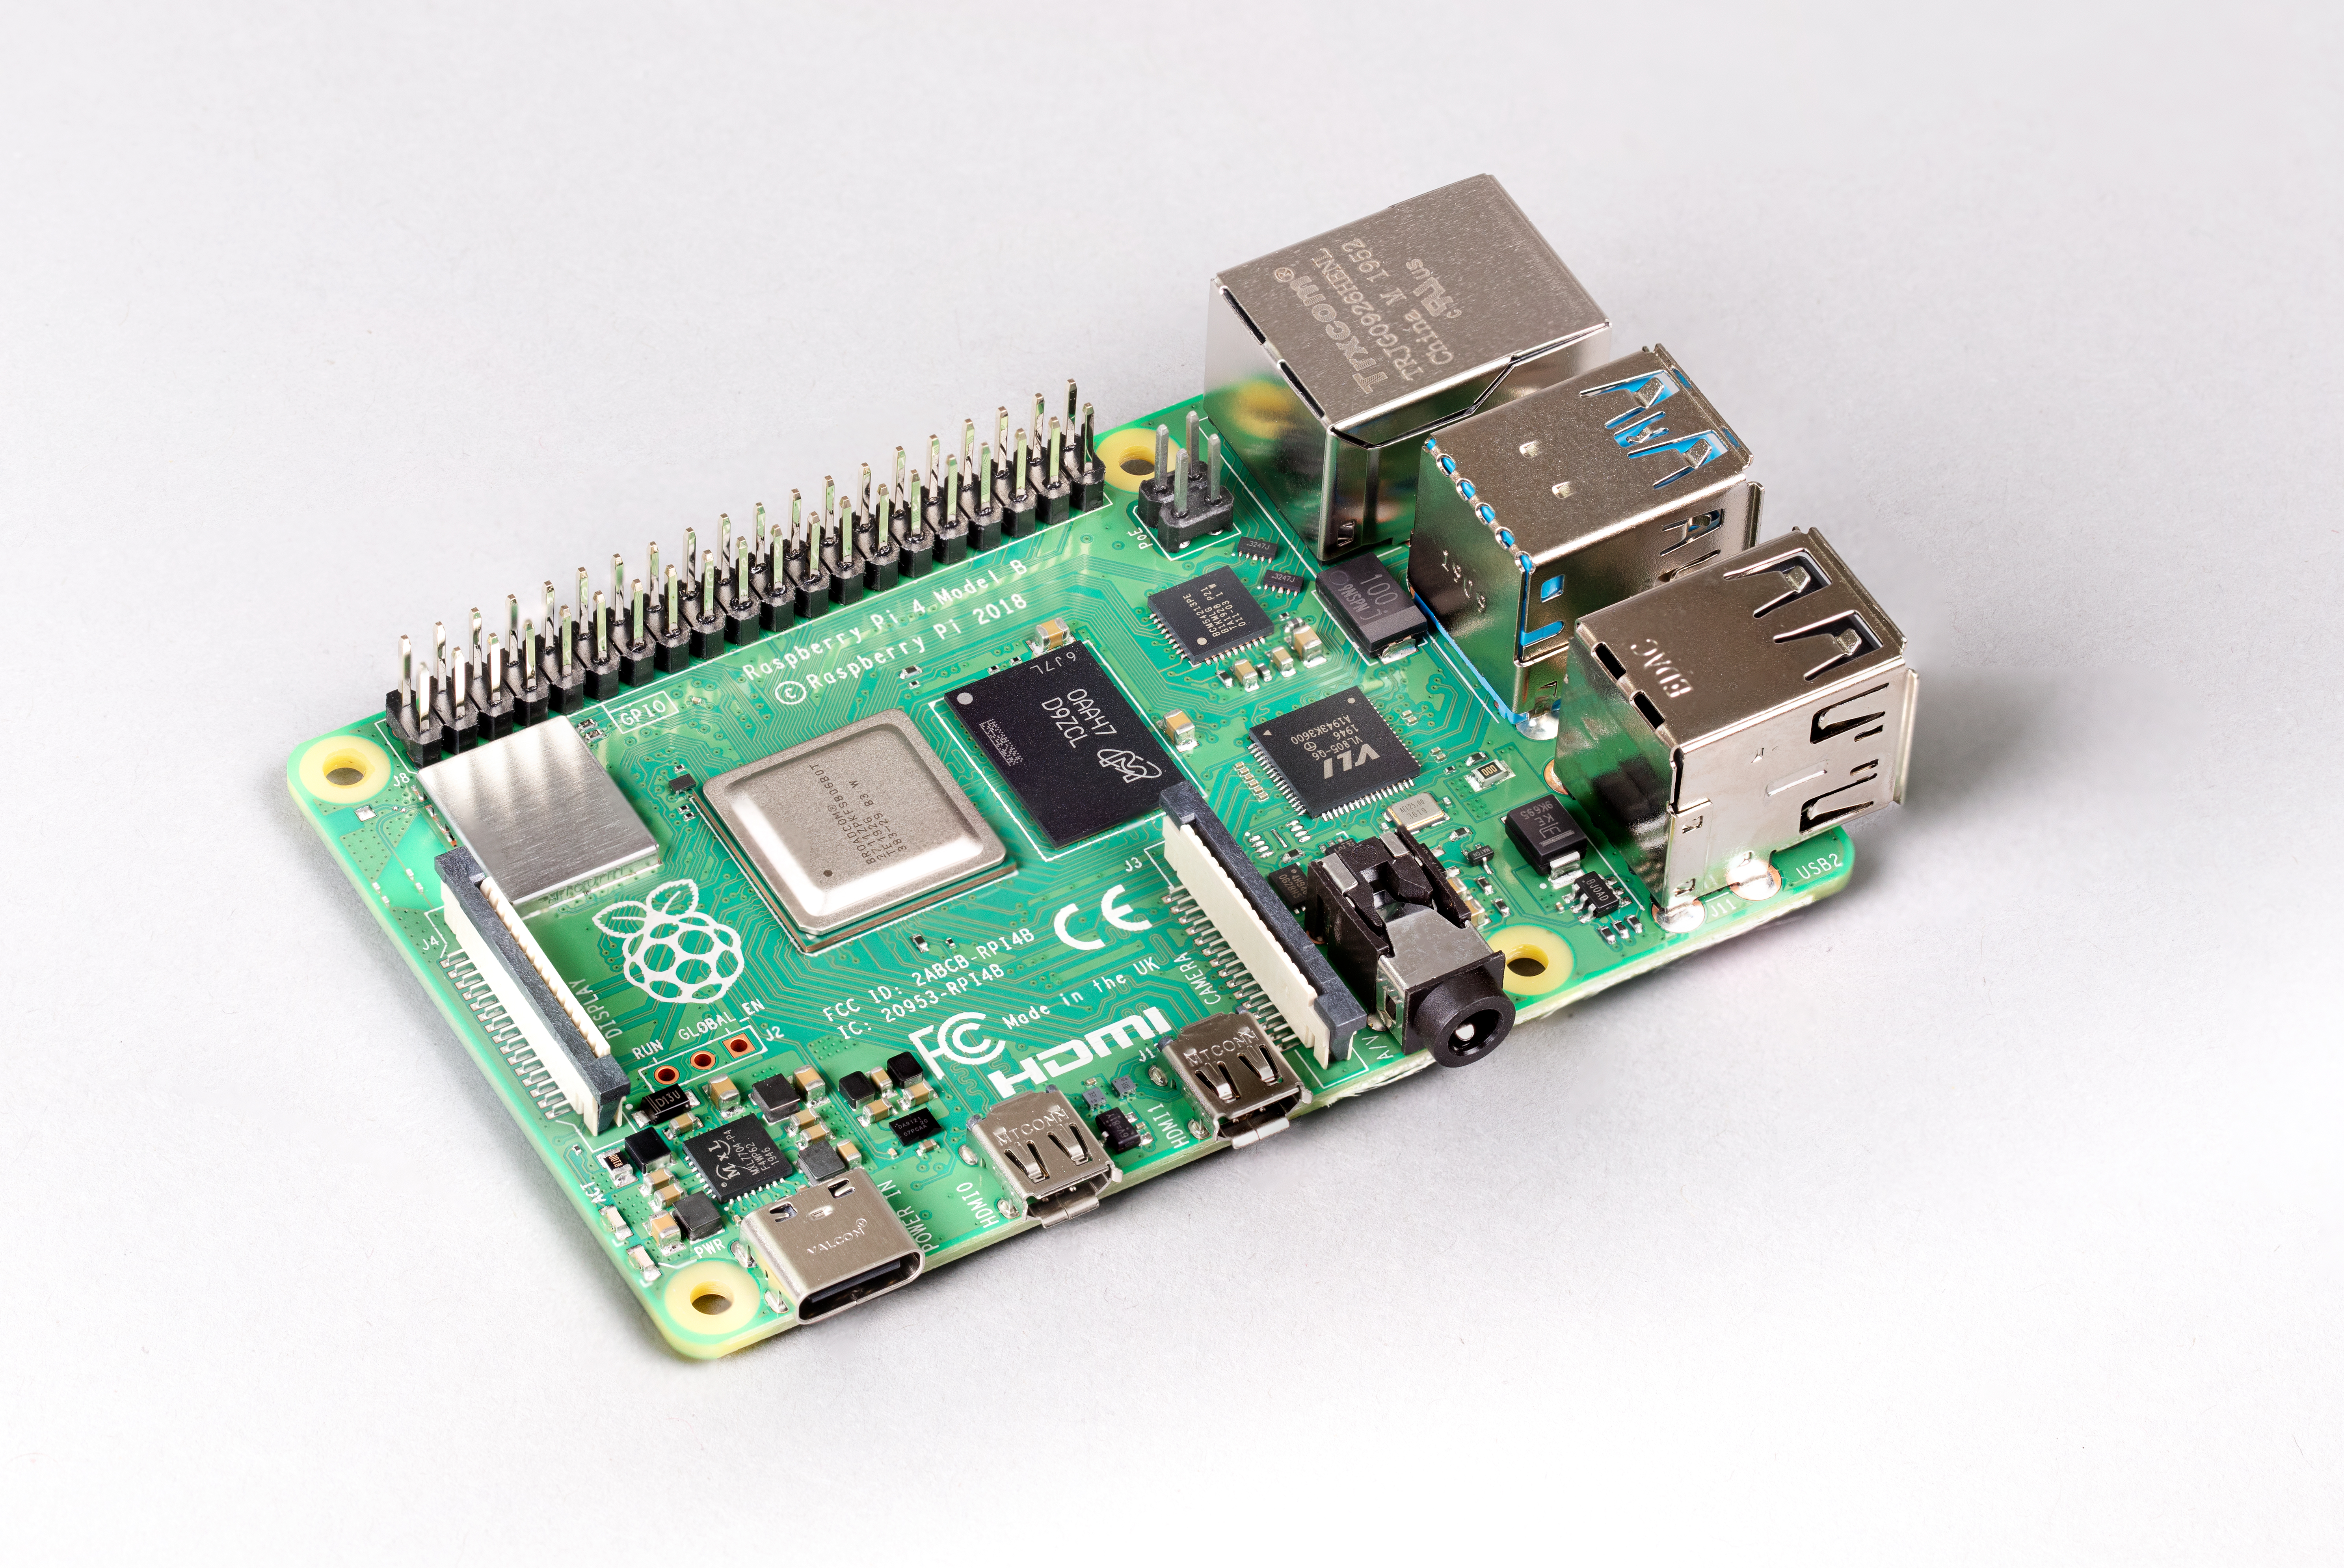
\includegraphics[width=0.4\textwidth,keepaspectratio]{img/rpi4b.jpg}
  \caption{Raspberry Pi 4 Model B}
  \source{Wikimedia Commons \cite{rpi4-side}.}
  \label{fig:rpi4b}
\end{figure}

\cleardoublepage

%%%%%%%%%%%%%%%%%%%%%%%%%%%%%%%%%%%%%%%%%%%%%%%%%%%%%%%%%%%%%%%%%%%%%%%%%%%%%%%%
%%%%%%%%%%%%%%%%%%%%%%%%%%%%%%%%%%%%%%%%%%%%%%%%%%%%%%%%%%%%%%%%%%%%%%%%%%%%%%%%
% DISEÑO E IMPLEMENTACIÓN %
%%%%%%%%%%%%%%%%%%%%%%%%%%%%%%%%%%%%%%%%%%%%%%%%%%%%%%%%%%%%%%%%%%%%%%%%%%%%%%%%

\chapter{Design and implementation}
\label{chap:design}

\section{System architecture}
\label{sec:sysarch}

\subsection{Top level}

\begin{figure}
  \centering
  \includegraphics[keepaspectratio]{img/toplevel-sysarch.png}
  \caption{Top level diagram of the hardware/software interactions \todo[inline]{Draft}}\label{fig:toplevel}
\end{figure}

The purpose of the Dronecontrol application is to be able to direct the movement of a \gls{uav} through the analysis of the images taken by a camera.
Since the processing power needed to work with the images recorded is superior to that offered by the autopilot flight controller it becomes necessary the use of an additional companion computer that will control the camera and employ machine learning to extract useful features from the images, as well as transform those features into movement directives for the vehicle.

A top level diagram of the individual parts that comprise the system is shown in Figure~\ref{fig:toplevel}. The main elements are the flight controller, that will run the PX4 autopilot \ref{subsec:px4}, the companion computer, that will run the developed application, and the camera, which provides the images.
The flight controller interfaces directly with the companion computer using the \gls{mavlink} protocol described in Section~\ref{subsec:mavlink}, either through a wireless radio link or a cabled serial connection between the two.
The camera is connected to the companion computer through a cable into an USB port on the computer.
Typically, the type of connection between the flight controller and the computer depends on the desired setup for the system so in the case where the camera, and therefore the companion computer, flies onboard the vehicle it is most convenient to use a direct wire connection between the two, as it provides a faster and more stable link. 
This onboard configuration is further detailed in Section~\ref{subsec:offboard}.
On the other hand, in the case where the companion computer will be acting more like a ground station on an offboard configuration it becomes strictly necessary to communicate with the flight controller through a wireless connection. For this purpose, a pair of telemetry radios provided with the Development Kit of the Holybro X500 (\ref{subsec:pixhawk}) are used. The complete setup requiered for this configuration is described in Section~\ref{subsec:onboard}.

In this project, the flight controller is driven by the PX4 software (\ref{subsec:px4}) and the hardware employed is optimized for this flight stack.
PX4 uses sensors to determine the vehicle state, which is needed for stabilization and to enable autonomous control.
It minimally requires a gyroscope, accelerometer, magnetometer (compass) and barometer.
A GPS or other positioning system is needed to enable all automatic flight modes, and some assisted ones.
PX4 uses outputs to control motor speed, flight surfaces like ailerons and flaps, camera triggers, parachutes, grippers, and many other types of payloads.
Many PX4 drones use brushless motors that are driven by the flight controller via an Electronic Speed Controller (ESC).
The ESC converts a signal from the flight controller to an appropriate level of power delivered to the motor.
PX4 drones are mostly commonly powered from Lithium-Polymer (LiPo) batteries.
The battery is typically connected to the system using a Power Module or Power Management Board, 
which provide separate power for the flight controller and to the ESCs for the motors.
A Radio Control (RC) system is used to manually control the vehicle.
It consists of a remote control unit that uses a transmitter to communicate stick/control positions with a receiver based on the vehicle.
Some RC systems can additionally receive telemetry information back from the autopilot.
Telemetry Radios can provide a wireless MAVLink connection between a ground control station and a vehicle running PX4.
This makes it possible to tune parameters while a vehicle is in flight, inspect telemetry in real-time, change a mission on the fly, etc.

On an actual UAV, the PX4 software runs on a dedicated piece of hardware like the Pixhawk 4 flight controller described in Section~\ref{subsec:pixhawk} that includes all the minimal required sensors for flight as well as interfaces to connect additional actuators and I/O systems (RC, telemetry radio, etc).
However, it is also possible to simulate this hardware on a standard Linux system by building the PX4 source code on a computer with this operating system.
This process is described in the development environment section (\ref{sec:devenv}).

The Dronecontrol application that runs on the companion computer has been developed using the Python programming language \footnote{\url{https://www.python.org/}}.
It offers good advantages for a project of this characteristics because of its high-level,
easy-to-use syntax, that usually results in a smaller code base than other comparable languages for small projects, its versatility and support for object-oriented programming. 
Most importantly, Python is widely used and its official package manager \gls{pip} greatly simplifies the use of external libraries and which gathers in its package index \footnote{\url{https://pypi.org/}} thousands of standard utilities,
including many machine learning and image processing projects and all the required libraries for interacting with PX4 through the MAVLink protocol (MavSDK).
As it is an interpreted language, it can run easily in any system with Python installed without the need to compile separate binaries for different operating systems.

The next sections explore deeper into the differences between the two configurations mentioned before: offboard computer (or ground station) and onboard computer.

\subsection{Offboard configuration}
\label{subsec:offboard}

The offboard configuration allows the flight controller to communicate and receive orders from a companion computer that is not physically connected to its hardware but that can instead stay on ground while the vehicle flies.
This has the advantage that it permits a simpler configuration, without having to be concerned with low-level hardware interactions between the two systems or powering of the companion computer while in flight, as well as allowing the use of a more powerful computer for image processing.
However, it also requires that the camera stays connected to computer on the ground so it cannot use images from the perspective of the drone in flight which limits the real-world applications of the system.
Other configurations involving a direct connection from a camera to the flight controller and the transmission of its images wirelessly to the companion computer through mavlink for processing can be feasible with the current technology but fall out of the scope of this project.

The wireless link is established in this instance through a pair of telemetry radios that connect to a telemetry port on the flight controller and to a USB port in the companion computer, respectively.
Since the Pixhawk 4 is configured by default to used its \verb|TELEM1| port for this purpose, no additional configuration is needed when using that port.
In the companion computer, applications like the QGRoundControl \footnote{\url{http://qgroundcontrol.com/}} ground station software which is part of the Dronecode Project are able to detect automatically a telemetry radio inserted into any of the USB ports of the host computer.
Additionally, other applications using the MavSDK (\ref{subsec:mavlink}) library can establish connection specifying the baudrate and the USB serial port address, usually something similar to \verb|/dev/ttyUSB0| on Linux and \verb|COM#| on Windows.

The radio used for the physical tests in this project is the Holybro SiK Telemetry Radio \footnote{\url{http://www.holybro.com/product/transceiver-telemetry-radio-v3/}}.
It is a small, light and inexpensive open source radio platform that typically allows ranges of better than 300m “out of the box” (the range can be extended to several kilometres with the use of a patch antenna on the ground).
The radios are offered either as 915Mhz (Europe) or 433Mhz (US) so they can be used in different regions and comply with the regulations for frequency, hopping channels and power levels.
They offer 2-way full-duplex communication through an adaptive TDM UART interface and their antenna allows for an adjustable 100-mW-maximum output power and -117 dBm receive sensitivity.
The link is established by default with a baudrate of 57600 (max bits per second on a serial channel) and it can provide air data rates of up to 250 kbps.

\todo[inline]{Images of the radios}
\todo[inline]{Images of the flight controller}
\todo[inline]{Connection diagram / pictures}

\subsection{Onboard configuration}
\label{subsec:onboard}

The second way of configuring the interaction between the flight controller and the companion computer consists of integrating both together on board the \gls{uav}.
In this case, the connection is done through a direct cable between the serial port in the flight controller and a USB port in the companion computer.
The camera will then be connected via cable as well to the companion computer and oriented in the vehicle in a way that allows for the best possible perspective during flight.
This configuration makes it possible to develop new control solutions based on images taken directly from the vehicle and that reflect the trajectory that it follows.
Therefore, it becomes possible to adjust the control loop based on previous reactions of the vehicle to commands and maintain a feedback loop for a more stable guidance.

Since the computer running the visual processing algorithm now has to fly on board the vehicle, it becomes specially important to make a good choice when selecting hardware.
To be able to take into the air, the computer has to be light enough that its weight can be lifted by the propellers while maintaining an adequate battery autonomy, but also powerful enough that the processor can handle the computer vision algorithms required to extract the necessary features from the images taken from the onboard camera that are to be feed to the control loop.

\begin{figure}
  \centering
  \includegraphics[width=\textwidth,keepaspectratio]{img/rpi4.png}
  \caption{The Raspberry Pi 4 microcomputer, with its 40-pin GPIO header marked in red}\label{fig:rpi4}
\end{figure}
\todo[inline]{Add pinout figure}
The Raspberry Pi 4 model chosen for this project and shown in Figure~\ref{fig:rpi4} is one of the most popular small computers available in the market at the time and it is widely use in all kinds of robotics projects both for education and hobbyists.
One of the most important advantages of using such a platform is the easy access to a great amount of manuals, guides and other support available online.
In addition, the Raspberry's officially supported operating system, called Raspberry Pi OS, is a Debian-based version of Unix optimized for its ARM microcontroller, which simplifies the process of moving from an Ubuntu test environment into real flight experiments.
Since this computer is designed to be easy to integrate with hardware projects it includes a 40-pin GPIO header (marked in red in Figure~\ref{fig:rpi4}) that can be programmed for connecting to any number of external devices.

The Raspberry Pi is powered by a 5V input that can be provided either from its USB-C port or through one of two pins in the header dedicated to this (marked as DC 5v power on Figure~\ref{fig:pinout}.
In the case of the particular vehicle build used in this project, the power management board used (the Holybro PM07 \footnote{\url{http://www.holybro.com/product/pixhawk-4-power-module-pm07/}}) also provides 5V to the flight controller, as well as powering the ESCs to the motors, and counts with two power outputs so one of them can be connected to the flight controller's \verb|POWER1| port and the other to the Raspberry Pi's pins through a custom-made connector.
\todo[inline]{Power management: more about this when it works}

In regards to the camera that will fly onboard the vehicle, there are many possibilities to chose from.
The most important characteristics that should be looked for are a small weight and simple plug-and-play interaction with the onboard computer.
For the tests carried out and detailed in Section~\ref{chap:validation} a Logitech 1080p webcam \todo{Exact model and link} has been used.
Since the frame of the Holybro X500 is not prepared by default to include an onboard camera, it became necessary to design a support to hang from the central rods of the vehicle frame where the camera could be attached securely during flight.
\todo[inline]{Pictures and 3D model}

\begin{figure}
  \centering
  \includegraphics[keepaspectratio]{img/wiring-diagram.pdf}
  \caption{A diagram of the wired connections from the Raspberry Pi 4 to the power management board (TELEM1) and the flight controller (TELEM2).}\label{fig:wiring}
\end{figure}
The second wired connection that needs to be established for this configuration is between the flight controller and the companion computer so the Mavlink messages can be exchanged.
As it is desirable to be able to maintain a wireless link to the vehicle even while it is being controlled by the onboard computer, the telemetry radio is kept connected to the \verb|TELEM1| port of the flight controller and the companion computer is wired to the \verb|TELEM2| port.
This port is not configured to be used by default so it is necessary to modify the configuration of the Pixhawk board either through QGroundControl \todo{More about QGC in SotA} or the PX4 console. \todo{More about this in validation ????}
The other end of the connector has three female Dupont wires that go into the TX/RX UART pins of the Raspberry Pi.
A diagram of the connections to the companion computer can be seen in Figure~\ref{fig:wiring}.
\todo[inline]{Description of 6 wires from connectors both power and telem}

In comparison with the default baudrate of 57600 on the telemetry radio link established in the previous section the wired serial connection works at a baudrate of 921600, which means the data is transferred 16 times faster through the link.
\todo{Main limitation is image processing though, so slower processing power from computer means slower responsiveness to movement all together. Any info about update rate from PX4? Does it depend on the link speed or is it constant?}
\todo[inline]{Link to section in validation where onboard setup is done}

The offboard configuration allowed the supervision of the output from the program while the vehicle was flying, since the computer stayed stationary on the ground, however in this configuration it is not possible to have a screen connected directly to the companion computer.
To fix this situation and be able to monitor during flight, as well as being able to give input directly to the program, it is possible to make use of the WiFi receptor of the Raspberry Pi to configure a remote desktop and connect to it through another computer serving as a ground station;
then the output from the camera and the image recognition can be seen in real time.
A more detailed description of the configuration required can be found on Section~\ref{sec:devenv}.

\section{Development environment and simulation}
\label{sec:devenv}
During the process of developing the application, it became necessary to be able to continuously deploy and test the latest version without having to depend on flying the physical vehicle, but instead relying on the simulation of the system inside the computer that was at the same time running the developed software.
This configuration has the twofold advantage of reducing the development time on the one hand, since there is no need to be concerned with the interactions between the different hardware components and the results can be visualized immediately in the computer screen, and on the other hand of increasing the safety of the process by only running on the vehicle software that has already been tested to an acceptable point.

Simulators allow PX4 flight code to control a computer modeled vehicle in a simulated "world" that can be interacted with in the same ways as with a real vehicle, using QGroundControl, an offboard API, or a radio controller/gamepad. PX4 supports two different simulation modes: software-in-the-loop (\gls{sitl}), where the flight stack runs on a computer, and hardware-in-the-loop (\gls{hitl}), where it uses a simulation firmware on a real flight controller board.
\begin{figure}
  \centering
  \includegraphics[width=\textwidth,keepaspectratio]{img/px4_simulator_messages.png}
  \caption{Mavlink messages exchanged between the simulator and the flight stack during simulation.}\label{fig:simulator-msgs}
\end{figure}
In both modes, the simulation works according to the feedback loop shown in Figure~\ref{fig:simulator-msgs}. 
The simulator generates the input from the sensors based on its internal world representation and sends it through Mavlink messages to the flight stack running on the same computer using the \gls{udp} transport protocol, which in turn generates response actuator controls that are fed back into the simulator in the same way to affect the vehicles position, velocity and attitude in the simulated world.
\todo[inline]{Explain more about how mavlink protocol works (messages) ???? On SotA ????}

There are many options for simulators supported by PX4 like Gazebo, a powerful 3D simulation environment for Linux systems that is particularly suited for testing object-avoidance and is commonly used with ROS, or AirSim (\ref{subsec:airsim}), a more resource-intensive cross-platform simulator that leverages the Unreal Engine, typically used for game development and animation to provides physically and visually realistic simulations.
For this project AirSim was chosen because of previous experience with Unreal Engine as well as for the easy availability of visual packages to test computer vision features and its native support for running on Windows machines, which is the operating system running on the computer where the tests will take place.
AirSim offers as well a Python library called airlib (\footnote{\url{https://pypi.org/project/airsim/}}) that can be used to retrieve images taken from a simulated camera from the perspective of the drone in the simulation world.
This feature will be necessary when testing the person-recognition utilities used in the program.
\begin{figure}
  \centering
  \includegraphics[width=\textwidth,keepaspectratio]{img/airsim-overview.png}
  \caption{High level overview of how different components interact with each other in the AirSim simulator.}\label{fig:airsim-overview}
\end{figure}
A high level overview of the simulator architecture and the way different components interact with each other can be seen in Figure~\ref{fig:airsim-overview}. 
The API layer present in the Figure inside the simulator environment refers to AirSim's own airlib library, which exposes with high-level functionality to send control commands to the flight controller directly.
However, in order to share the same control code when simulating flight and in real flight without and not depend on the simulator system, the control commands are sent using the official MavSDK API instead, which allows communication of estimated state, desired state and sensor data directly between the flight controller firmware and the companion computer.

In order to run software-in-the-loop simulation, the PX4 firmware needs to be built from the source code on the Linux platform where it is going to run.
The build system then sets up all the necessary ports for the Mavlink communication and starts a local instance of the NuttX operating system that runs on the actual flight board.
\begin{figure}
  \centering
  \includegraphics[width=\textwidth,keepaspectratio]{img/px4-ports.png}
  \caption{Network diagram between the different components that interconnect during software-in-the-loop simulation.}\label{fig:px4-ports}
\end{figure}
Figure~\ref{fig:px4-ports} shows how the different parts of the system communicate with each other inside a SITL simulation.
PX4 uses commonly established UDP ports for MAVLink communication with ground control stations (e.g. QGroundControl), offboard APIs (e.g. MAVSDK, MAVROS) and simulator APIs (e.g. AirSim, Gazebo).
External developer application like Dronecontrol use an offboard API, in this case MAVSDK, and therefore listen to PX4's remote UDP port 14540.
All ports in the range 14540-14549 can be used to connect offboard API, for example in the case of controlling multiple vehicles at the same time.
PX4's remote UDP Port 14550 is used for communication with ground control stations, which are expected to listen for connections on this port (QGroundControl listens to this port by default).
PX4 uses a simulation-specific module to connect to the simulator's local TCP port 4560. 
Simulators then exchange information with PX4 using the Simulator MAVLink API shown in Figure~\ref{fig:simulator-msgs}. 
PX4 on SITL and the simulator can run on either the same computer or different computers on the same network.

Since the purpose of using AirSim as a simulator is to run it on a Windows computer and the PX4 software-in-the-loop stack runs on Linux, it is necessary to run a virtualized Linux OS in parallel on the Windows computer and setup a local network so that the simulator and the flight controller firmware can communicate with each other.
The PX4 development team officially supports running the SITL flight stack in Windows through the Windows Subsystem for Linux (WSL2)\footnote{\url{https://docs.microsoft.com/en-us/windows/wsl/about}}, which allows users to install and run their Ubuntu Development Environment on Windows as if it was running it on a Linux computer.
The Windows Subsystem for Linux lets developers run a GNU/Linux environment (including most command-line tools, utilities, and applications) directly on Windows, unmodified, without the overhead of a traditional virtual machine or dualboot setup.
The full steps needed for to configure the system are detailed in Section~\ref{sec:test2}.

\begin{figure}
  \centering
  \includegraphics[scale=0.8,keepaspectratio]{img/sitl-connections.png}
  \caption{Connection diagram of how the three systems that interact with each other during SITL simulation.}\label{fig:sitl-connections}
\end{figure}
The whole set of connections established in the software-in-the-loop simulation is shown in Figure~\ref{fig:sitl-connections} at the transport layer level. The two systems that run inside the virtualized Linux system through WSL (the simulated flight stack and the dronecontrol program) connect through the localhost network on the UDP port defined by PX4 for Offboard APIs and each of them connects in turn to the AirSim simulator through the virtual Local Area Network established by the Windows Subsystem for Linux to the host Windows computer.
The PX4 flight stack on SITL mode connects to the simulator using the TCP port 4560, as defined by PX4 on Figure~\ref{fig:px4-ports}, and dronecontrol connects through the AirSim library which uses by default a TCP connection on port 41451.

In the case of hardware-in-the-loop simulation, the main difference with SITL is that the flight stack firmware runs on a physical flight board using a special configuration.
In HITL all motors/actuators are blocked, but internal software is fully operational.
This configuration adds an additional separated operating system and to make this mode of testing simpler, since the WSL environment is no longer needed to run the flight stack, it is possible to move the execution of the Python module to Windows.
This eliminates the need to add further configuration to allow the external flight controller to communicate with the internal WSL network, which is by default only accessible by its Windows host computer.
Moreover, now that PX4 runs on a separate piece of hardware, it is necessary to establish two separate physical connections to the Windows computer, so that both the simulator and the Python app can communicate through their own channel to the flight controller, either wired, to the microUSB port or an unused telemetry port on the flight controller, or wireless through a telemetry radio.

\begin{figure}
  \centering
  \includegraphics[scale=0.8,keepaspectratio]{img/hitl-connections.png}
  \caption{Connection diagram of how the three systems that interact with each other during HITL simulation.}\label{fig:hitl-connections}
\end{figure}
Figure~\ref{fig:hitl-connections} shows the chosen connections to execute tests in HITL mode.
The Windows machine runs both AirSim and the Python interpreter, which communicate through the localhost network using \gls{TCP}.
The board running PX4 connects to the simulator through a USB to microUSB cable, which is setup to work with a baudrate of 115200, and to the developed program through a telemetry radio running at a baudrate of 57600, both attached to USB ports on the Windows computer accessible through their COM address.

\section{Software architecture}

\begin{figure}
  \centering
  \includegraphics[width=12cm, keepaspectratio]{img/code_diagram.jpg}
  \caption{Structure of the program}\label{fig:architecture}
  \todo[inline]{Draft (use miro for final??)}
\end{figure}

Figure~\ref{fig:architecture} shows the main modules the designed the software is composed of and how it interacts with the external libraries.
The application consists of three basic parts: 
the pilot module, in charge of sending instructions to the flight controller and receiving back information on position and state through the \verb|mavsdk| library, 
a video source module that handles the retrieval of images from different sources and the necessary processing for image analysis, 
and a control module that directs the interaction between the other two to transform the pixel information first into position points through the \verb|mediapipe| library and then into instructions for the pilot.
The upper part of the diagram in Figure~\ref{fig:architecture} shows how the program modules receive input and send instructions to the hardware systems whether these are simulated or not.
Other smaller utilities have also been developed to help test how the systems interact with each other and calibrate different parts of the control behaviour.
\todo[inline]{Command-line interface summary here and link to appendix with full help extract.}
These different parts that make up the dronecontrol app are detailed in the next sections.

\subsection{Pilot module}
The purpose of the pilot module is to provide access to the rest of the application to send and receive messages from the PX4 controller through the MavSDK library.
This library provides a simple asynchronous API for managing one or more vehicles, providing programmatic access to vehicle information and telemetry, and control over missions, movement and other operations.
MavSDK utilizes the python standard library \emph{asyncio} to be able to run coroutines in parallel while waiting for the messages provided through the \emph{MAVLink} communication.
Therefore all calls to the library have to be written as async functions that await the result of one or more polls to the flight stack.

\verb|asyncio| provides support for writing concurrent code using the \verb|async/await| syntax.
It is used as a foundation for multiple Python asynchronous frameworks that provide high-performance network and web-servers, database connection libraries, distributed task queues, etc; 
and provides a set of high-level APIs to run Python coroutines concurrently and have full control over their execution.
The pilot module integrates \verb|mavsdk| and \verb|asyncio| and provides a queue for the control module to send actions to be executed in the vehicle one after another.

Listing~\ref{lst:pilot.connect} shows how to establish a connection to a PX4 vehicle through its physical (serial) or virtual (UDP) address and poll for internal information from the flight controller to decide when the system is ready to receive instructions.
The mavsdk library exposes telemetry and other state information through asynchronous generators, which are defined in python as a convenient way to make asynchronous data producers and accessed with the \mintinline{python}{async for} syntax.


\begin{listing}[h!]
    \caption{Example of how the communication to the flight stack is established through asyncio and the mavsdk library}{}
    \label{lst:pilot.connect}
    \begin{minted}[breaklines, fontsize=\footnotesize, baselinestretch=1]{python}
async def connect(self):
    """Connect to mavsdk server.
       Raises a TimeoutError if it is not possible to establish connection.
    """
    
    if self.serial:
        address = f"serial://{self.serial}"
    else:
        address = f"udp://{self.ip if self.ip else ''}:{self.port}"
    self.log.info("Waiting for drone to connect on address " + address)
    await asyncio.wait_for(self.mav.connect(system_address=address), timeout=self.TIMEOUT)

    async for state in self.mav.core.connection_state():
        if state.is_connected:
            break

    # Wait for drone to have a global position estimate
    async for health in self.mav.telemetry.health():
        if health.is_global_position_ok:
            break
        
    self.log.info("System ready")
    self.is_ready = True
    \end{minted}
\end{listing}

Many of basic operations that can be executed in the flight controller are implemented in the pilot module with error handling and safety checks, like takeoff, landing, return home or manipulating the vehicle flying velocity directly by providing speeds in body coordinates.
These actions can be executed directly or added to a queue that runs in on a loop executing them in the order they are added, waiting until the previous action has finished and the vehicle is in the desired state before starting the next.
The loop that runs this queue can be seen in Listing~\ref{lst:pilot.queue}.
There is a maximum time of 10 seconds that each action can use to run
The loop stops when the asynchronous task it runs on is cancelled with \mintinline{python}{task.cancel()}, which raises a \mintinline{python}{CancelledError} exception in the parallel execution.

\begin{listing}[h!]
    \caption{Loop where the action queue runs on the pilot module. Each action is awaited until it finishes or the timeout time runs out.}{}
    \label{lst:pilot.queue}
    \begin{minted}[breaklines, fontsize=\footnotesize, baselinestretch=1]{python}
async def run_queue(self):
    """
    Run the queue loop.
    
    Queued actions will be awaited one at a time
    until they are finished.
    The loop will sleep if the queue is empty.
    """
    try:
        while True:
            if len(self.actions) > 0:
                action = self.actions.pop(0)
                self.log.info("Execute action: %s", action.func.__name__)
                try:
                    await asyncio.wait_for(action.func(self, **action.args), timeout=10)
                except asyncio.exceptions.TimeoutError:
                    self.log.warning(f"Time out waiting for {action.func.__name__}")
            else:
                await asyncio.sleep(self.WAIT_TIME)
    except asyncio.exceptions.CancelledError:
        self.log.warning("System stop")
    \end{minted}
\end{listing}

\subsection{Video source module}

The objective of the video source module is to provide a collection of classes to retrieve images from different sources,
in a way that they can be exchanged for one another without affecting the rest of the application to facilitate testing and be adaptable running in different environments.
There are three classes of video sources implemented: file, simulator and camera, which inherit from the same \mintinline{python}{VideoSource} base class as shown in Figure~\ref{fig:video-source-inheritance}.

\begin{figure}
  \centering
  \includegraphics[width=8cm, keepaspectratio]{img/placeholder.png}
  \caption{Diagram of inheritance on the video source classes available to retrieve image data.}\label{fig:video-source-inheritance}
  \todo[inline]{Make inheritance schema}
\end{figure}

The \mintinline{python}{FileSource} class is able to open a video file stored in the companion computer and provides images taken frame by frame from it until the video ends.
This allows the program to replay the image detection algorithms on videos previously captured by the camera tool exposed in section~\ref{subsec:test-tools}.
The \mintinline{python}{CameraSource} class can access a physical camera attached to the computer running the application via USB and provide the frames captured in real time.
Both the file and camera sources employ OpenCV's video capture utilities to take care of the file handling and the camera driver management capabilities respectively.

The simulator source uses AirSim's Python library to communicate with the simulator and retrieve images from a simulated camera attached to the 3D model of the vehicle in Unreal Engine.
It connects automatically through localhost, but it can also be provided with an IP to establish connection to the simulator running on a different computer on the local network, for example when the program runs inside WSL and the simulator runs on its host computer.

\subsection{Control module}
The control module contains the main logic of the application and is in charge of converting the raw images obtained from the video source into commands for the pilot module.
Two different types of control have been implemented.
The first one is a proof-of-concept control solution, described in Section~\ref{subsec:hands}, that runs in offboard mode (see Section~\ref{subsec:offboard}) and translates some predefined hand gestures into simple commands for the aerial vehicle, of which the main purpose is to be able to test the interaction between all the components of the system in a more easily controlled environment, since it uses the simpler configuration of situating the computer with the controller outside of the vehicle.
The second control system consists of a follow solution more applicable to real-life scenarios where the control and the camera is onboard the vehicle and the presence of a person is detected in the images obtained from the perspective of the drone in order to be able to give the flight controller velocity commands to follow said person and maintain it centered in its view.

The process followed in both solutions consists roughly of the same two parts.
First the image is sent to the computer vision and machine learning third-party library that extracts the required features from the image in the form of 2D coordinates.
Afterwards a series of calculations depending on the particular solution are applied to these coordinates to decide which commands are sent to the pilot module.
The third-party library used for computer vision in the program is the mediapipe library described in Section~\ref{subsec:mediapipe}, which offers cross-platform, customizable ML solutions for live and streaming media, specifically its hand and pose detection solutions.

To engage the module in direct control of the vehicle's velocity it is necessary to use a special flight mode defined by PX4 for this purpose, called Offboard Mode \footnote{\url{https://docs.px4.io/main/en/flight_modes/offboard.html#offboard-mode}} (not to be confused with the offboard configuration described in section~\ref{subsec:offboard}).
Offboard mode is primarily used for controlling vehicle movement and attitude, and supports only a very limited set of MAVLink messages. This mode requires position or pose/attitude information to be available to the flight controller, e.g. GPS.
In it, the vehicle obeys a position, velocity or attitude setpoint provided over MAVLink by a MAVLink API (i.e. MAVSDK) running on a companion computer and usually connected via serial cable or wifi.
A stream of setpoint commands must be received by the vehicle at a rate higher than 2Hz prior to engaging the mode and in order to remain in it.
If the message rate falls below 2Hz or the connection is lost the vehicle will stop and, after a timeout, the vehicle will attempt to land or perform some other failsafe action according to the parameters configured.
In order to hold position while in this mode, the vehicle must receive a stream of setpoints for the current position.

The next two sections offer a more complete explanation of the control module used by the two different solutions developed.



\subsection{Proof of concept: hand-gesture solution}
\label{subsec:hands}
The main purpose of this solution is to test that the flow of the application works as expected, both in simulation and in real flight, and that all the systems are capable of establishing the required connections with each other.
For that reason it is designed to be able to be run in real flight with the minimal setup of a built drone with its default components and any computer with a webcam.

\begin{figure}
  \centering
  \includegraphics[width=\textwidth, keepaspectratio]{img/hand_landmarks.png}
  \caption{Landmarks extracted from detected hands by the MediaPipe hand solution}\label{fig:hand-landmarks}
\end{figure}

This control module runs on a loop that continuously polls for a new frame from the chosen video source and feeds it to the hand detection functionality from MediaPipe.
If a hand is detected in the images, 2D coordinates are extracted according to the map shown in Figure~\ref{fig:hand-landmarks}.
These landmarks are then converted into different discrete gestures like open palm, closed fist or an specific finger pointing different directions.
When a new gesture is detected, the command assigned to it is queued to the pilot module and executed as soon as the previous commands end their execution.

The conversion between landmarks and gestures is performed by drawing vectors from the base of each of the fingers to their tips as well as from the base of the hand (wrist feature) to the base of the fingers and using the dot product vector operation to calculate the relative angles between each finger and the base of the hand, as shown in Figure~\ref{fig:vector-calcs}.
By comparing the calculated angles to a threshold, it is possible to detect whether each individual finger is extended or folded, as well as the general direction it is pointing towards.
The open hand gesture, for example, can then be defined as all five fingers extended, that is, all five vectors defined by the fingers sharing the same approximate angle with the vector from the base of the hand to that finger.

\begin{figure}
  \centering
  \includegraphics[width=8cm, keepaspectratio]{img/placeholder.png}
  \caption{Vector calculations}\label{fig:vector-calcs}
\end{figure}

The full list of gestures detected by the program by calculating these angles is as follows:
\begin{itemize}
    \item No hand: happens when no landmarks are able to be extracted from the image. As a safety feature, in this case the vehicle stops whichever previous commands it had in its queue and goes into hold flight mode, where it just hovers in the air maintaining its position.
    \item Open hand: it is detected when all five fingers are extended, as if gesturing stop, and makes the drone land at its current position.
    \item Fist: it is detected when all five fingers are folded and makes the drone arm and takeoff. If the drone is already in the air nothing happens.
    \item Index finger pointing up: it is detected when only the index finger is extended and it is pointing roughly towards the top of the image ($\pm 30$ degrees) and makes the drone go into offboard mode, where it is possible to receive direct velocity commands.
    \item Index finger pointing to the right: same as above but pointing to the right of the image and makes the drone roll towards its right side at a speed of 1 m/s.
    \item Index finger pointing to the left: same as above but the drone rolls towards its left side.
    \item Thumb pointing to the right: it is detected when index finger is extended up (to maintain the drone in offboard control) and the thumb is extended pointing towards the right of the screen. This gesture makes the drone pitch forward at a steady speed of 1 m/s.
    \item Thumb pointing to the left: same as the previous gesture, but the drone pitches backward when the thumb point to the left of the screen.
\end{itemize}

\todo[inline]{Include some code for the module after cleanup, vector calcs and/or running loop}
\todo[inline]{Include diagram of angles for each pointy gesture ?????}
\todo[inline]{Include images of program output image with drawn lines for gestures}


\subsection{Final solution: human following}
\label{subsec:follow}

\subsection{Other utilities}
\label{subsec:test-tools}


\cleardoublepage

%%%%%%%%%%%%%%%%%%%%%%%%%%%%%%%%%%%%%%%%%%%%%%%%%%%%%%%%%%%%%%%%%%%%%%%%%%%%%%%%
%%%%%%%%%%%%%%%%%%%%%%%%%%%%%%%%%%%%%%%%%%%%%%%%%%%%%%%%%%%%%%%%%%%%%%%%%%%%%%%%
% EXPERIMENTOS Y VALIDACIÓN %
%%%%%%%%%%%%%%%%%%%%%%%%%%%%%%%%%%%%%%%%%%%%%%%%%%%%%%%%%%%%%%%%%%%%%%%%%%%%%%%%

\chapter{Experiments and validation}
\label{chap:validation}

This chapter contains...
\todo[inline]{Add flow diagram of testing process and sum up}
\todo[inline]{Add connection diagrams to each of the testing section below}

\section{PX4 SITL simulation and validation}
\label{sec:test-2-sitl}

Section \ref{sec:devenv} describes the software-in-the-loop simulation mode developed by PX4.
By using this mode, it is possible to test and validate the correct operation of each individual part in the program's architecture.
To begin with, it is necessary to validate that it is possible to use the connection between the simulated flight controller and the dronecontrol program to send commands to the simulated vehicle, as well as being able to capture images from a connected camera and use them to test the detection algorithm.
The full list of validation steps is therefore:
\begin{enumerate}
    \item Verify that it is possible to start the simulated flight controller and that it connects to the 3D simulator vehicle.
    \item Connect the dronecontrol program to the flight controller and send basic commands.
    \item Retrieve images from a camera and run computer vision detection on them.
    \item Integrate the last three steps by running the hand-gesture control solution described in section \ref{sec:hands}
\end{enumerate}

For this purpose and to be able to run with a minimal configuration, the Gazebo simulator \footnote{\url{https://gazebosim.org/home}} included with the base PX4 installation will be used as the 3D environment.
This simulator works inside Linux in the same computer that runs the SITL PX4.
To be able to later transition into using the AirSim simulator instead, which runs in Windows, with minimal changes, for this test PX4, Gazebo and the dronecontrol program will run inside the Windows Subsystem for Linux.
The complete installation process necessary to run these tests is explained in appendix \ref{app:install-px4} and \ref{app:install-dronecontrol}.

\begin{figure}
  \centering
  \includegraphics[width=.8\textwidth, keepaspectratio]{img/gazebo.png}
  \caption{Gazebo simulator (left) and output from the PX4 terminal (right) after PX4's software-in-the-loop mode is started}\label{fig:gazebo}
\end{figure}

Once both parts are installed, PX4 and Gazebo can be started by running the \mintinline{bash}{make px4_sitl gazebo} command inside its installation folder.
The result of this command can be seen in figure \ref{fig:gazebo}, where the left part shows the user interface and 3D world of the Gazebo simulator and the right side contains the PX4 console that can be used for sending commands and changing the configuration parameters of the simulated flight controller.
The simplest command to test is takeoff, which is done by sending \texttt{commander takeoff} through the console.
Figure \ref{fig:gazebo-takeoff} shows the state of the simulator after the takeoff command, with the vehicle model having climbed to the default height of 2.5 meters above ground.
To land the vehicle again, the command is \texttt{commander land}.

\begin{figure}
  \centering
  \includegraphics[width=.8\textwidth, keepaspectratio]{img/gazebo-takeoff.png}
  \caption{Gazebo simulator (left) and output from the PX4 terminal (right) after the takeoff command has been executed}\label{fig:gazebo-takeoff}
\end{figure}

The next step is to connect the dronecontrol application.
The camera testing tool described in section \ref{subsec:cam-tool} has been developed for this test, so that it is possible to establish a connection to PX4 SITL and process images without engaging any of the program's control modules.
The commands are then sent to PX4 through keyboard input, for example, the key "T" can be used to make the simulated vehicle take off.
Figure \ref{fig:sitl-hand} shows the image and text output of the program when the test camera tool is run with the hand detection feature activated.
On the left side, the detection algorithm tracks the joint of the hand present in the captured image and on the right side the logged information shows when the connection is established and keyboard commands are sent to the simulator.

\todo[inline]{Figure \ref{fig:sitl-hand}: Get a better image for this}
\begin{figure}
  \centering
  \includegraphics[width=\textwidth, keepaspectratio]{img/sitl-hand-2.png}
  \caption{Hand detection algorithm running on images taken from the computer integrated webcam}\label{fig:sitl-hand}
\end{figure}

The full execution of a test of the hand-gesture based control solution is shown in this \href{https://l-gonz.github.io/tfg-giaa-dronecontrol/videos/test-sitl-hand}{video}\footnote{\url{https://l-gonz.github.io/tfg-giaa-dronecontrol/videos/test-sitl-hand}} in this link and an image extracted from it can be seen in figure \ref{fig:sitl-hand-video}.

\begin{figure}
  \centering
  \includegraphics[width=\textwidth, keepaspectratio]{img/video-hand-sitl.png}
  \caption{Single frame from the video showing the full execution of the hand-gesture control solution}
  \label{fig:sitl-hand-video}
\end{figure}


\subsection{PX4 SITL validation with AirSim}
\label{sec:test-3-airsim}

The end goal for the testing environment is for it to use the AirSim simulator to be able to take advantage of its 3D-world and computer vision capabilities.
For this reason, it becomes necessary to validate that the new simulator can run correctly on Unreal Engine on the computer and interact with PX4 as well as it did with the default Gazebo simulator and that all the necessary features for detection, tracking and following work as expected.
All these characteristics will be checked in the order below:
\begin{enumerate}
    \item Verify that the AirSim simulator is able to start, connect to the PX4 SITL through the WSL virtual network and receive commands from the PX4 terminal.
    \item Check that the dronecontrol program can connect to both AirSim through the WSL network to receive images and PX4 through the local network to send movement commands.
    \item Test the pose recognition algorithms on the images obtained from the AirSim simulation.
    \item Check that the follow solution is able to control the velocity of the vehicle directly in PX4's offboard mode.
\end{enumerate}

In the first place, the AirSim simulator needs to be installed in the Windows host.
The full installation process is described in appendix \ref{app:install-airsim}.
There are specific configuration parameters that have to be set to be able to connect the AirSim simulator in Windows to the PX4 SITL running inside WSL.
On the simulator side, AirSim's settings file has to include a line defining the IP address of the network interface to use.
This parameter, along with the full configuration file used for SITL testing can be found on appendix \ref{app:airsim-config}.
On the PX4 side, it is necessary to specify that the simulator will attach through a different IP address than \texttt{localhost}.
This is done by setting the \texttt{PX4\_SIM\_HOST\_ADDR} environment variable in the Linux system to the IP address of the Windows host on the WSL virtual network before starting PX4 as follows:
\begin{minted}{bash}
export PX4_SIM_HOST_ADDR=[IP-address]
make px4_sitl none_iris
\end{minted}
This starts the software-in-the-loop execution, which attempts to attach to an already running simulator listening on the IP address specified and the TCP port 4560, in this case, AirSim.
Therefore, every time one of PX4 or AirSim stops its execution, both of them have to be restarted in the specific order of first the AirSim simulator and then the PX4 flight controller.
Figure \ref{fig:airsim-sitl} shows the testing environment after the AirSim simulator and the PX4 console have been started successfully.

\begin{figure}
  \centering
  \includegraphics[width=\textwidth, keepaspectratio]{img/airsim-sitl.png}
  \caption{AirSim environment connected to PX4 flight stack running in SITL mode}
  \label{fig:airsim-sitl}
\end{figure}

At this point, it is possible to use the PX4 console to send takeoff and land commands to the simulator and observe the 3D-model of the vehicle climb into the air.
To test the detection and tracking of human figures from images taken inside the simulator, one can again use the camera testing tool provided with dronecontrol.
Figure \ref{fig:airsim-sitl-pose} shows the output when the tool is run with the command:
\mint{bash}{dronecontrol tools test-camera --wsl --sim --pose-detection} 
and a 3D model of a person is situated in front of the drone in the simulated world.
In the image, the computer vision utilities detect the main features of the human body and a bounding box is drawn around it.
Meanwhile, the logged output from the program shows two calculated positions in the terminal: the x coordinate of the mid point of the bounding box and the percentage of the image height covered by the height of the bounding box.
These two numbers are the inputs for the PID controllers used in the follow solution as described in section \ref{sec:follow}, so that the output can be used to calibrate the distance from which the drone is to follow the person when that control mode is engaged.

\begin{figure}
  \centering
  \includegraphics[width=\textwidth, keepaspectratio]{img/airsim-sitl-pose.png}
  \caption{AirSim, PX4 and dronecontrol applications running side-by-side and connecting to each other}
  \label{fig:airsim-sitl-pose}
\end{figure}

Now that the testing environment is working as expected and before it is used to tune the PID controllers in the follow solution to the response of the vehicle's movement in the next section, it is possible to verify that the controllers are capable of reacting to changes in the position of the figure by only enabling their proportional term with an appropriately low magnitude to keep the movement slow and smooth.
The drone movement when running the follow control program with values of 10 and 2 on the proportional term of the yaw and forward controllers, respectively, which can be done with the command \mintinline{bash}{dronecontrol follow --sim --yaw-pid (10, 0, 0) --fwd-pid (2, 0, 0)}, is shown in video in this \href{https://l-gonz.github.io/tfg-giaa-dronecontrol/videos/test-sitl-follow}{link}\footnote{\url{https://l-gonz.github.io/tfg-giaa-dronecontrol/videos/test-sitl-follow}} and a frame extracted from it can be seen in figure \ref{fig:airsim-test-follow}.

\begin{figure}
  \centering
  \includegraphics[width=\textwidth, keepaspectratio]{img/video-follow-sitl.png}
  \caption{Single frame from the video showing the movement of the drone in response to changes in the position of the tracked person}
  \label{fig:airsim-test-follow}
\end{figure}
\clearpage

\section{PID controller validation}
\label{sec:test-1-pid}

% Process of tuning the PIDs
% Graphs from test-controller
% Analysis of error

\todo[inline]{Flow chart of validation process}
\todo[inline]{Videos for github}

As has been mentioned before, the velocity controller that is the heart of the person following mechanism is based on two PID controllers.
In order to get velocity outputs for the PID controllers that produce a stable movement of the vehicle, it is necessary to tune the parameters of the controllers until the appropriate combination is found.
The value for the coefficients used for the project has been found empirically with the help of the tuning tool described in section~\ref{subsec:test-tools} and developed for this purpose, and its performance validated with the controller testing tool, both running in a simulated environment with the flight stack in SITL mode so that it is possible to take continuous measures of the response of the PID controllers to step movements of a simulated person present in the 3D world.
In the first place, each of the controllers has been tuned independently of the other by allowing the vehicle only one direction of movement at a time.
Afterwards, both controllers are engaged at the same time to take measurements of their joint response to a range of different inputs.

The controllers are calibrated for a starting position of x=0, y=0 for the vehicle and x=600, y=0 for the person in world coordinates of the simulated environment.
At these position, the processing of the images taken from the simulated camera detects the person centered in the field of view and with a height of 36\% of the image height.
The set points for the controllers running in the simulator are therefore 0.5 for the yaw controller and 0.36 for the forward controller.

\subsection{Yaw controller}

\begin{figure}
  \centering
  \includegraphics[width=\textwidth, keepaspectratio]{img/4.1-tune/sim_window_tune.png}
  \caption{Starting position of the simulator for tuning the yaw controller}\label{fig:sim_window_tune}
\end{figure}

\begin{figure}
  \centering
  \includegraphics[width=.5\textwidth, keepaspectratio]{img/4.1-tune/yaw_tune_start_pos.png}
  \caption{Perspective from the vehicle at the start of the program run}\label{fig:sim_camera_tune}
\end{figure}

To find the correct coefficients for the controller that governs the yaw velocity of the vehicle, the target person is set in a position slightly to the side on its field of view so that when the controller is engaged it produces a rotation of the vehicle to that side.
Figure~\ref{fig:sim_window_tune} shows the starting position of the simulated environment before each run, where the 3D model has been situated at (600,50), that is, 50 units to the right of the target position.
The image captured from the simulated camera is shown in figure~\ref{fig:sim_camera_tune}.

\begin{figure}
  \centering
  \includegraphics[width=.45\linewidth]{img/4.1-tune/yaw_p1_feedback.pdf}
  \includegraphics[width=.45\linewidth]{img/4.1-tune/yaw_p1_speed.pdf}
  \caption{Variation of (a) input position and (b) output velocity for different values of $K_{P}$ while the yaw controller is engaged.}\label{fig:tune-yaw-prop}
\end{figure}


The first step taken is to test different values of $K_{P}$ while maintaining $K_{I}$ and $K_{D}$ at zero.
Figure~\ref{fig:tune-yaw-prop} shows the output of the tuning program for the tested values of $K_{P}$.
The left graph represents the variation of the horizontal position detected by the camera for the first 10 seconds after activating the controller and the right graph, the velocity that the controller outputs to the pilot module to reach the target.
It can be seen that for low values of $K_{P}$, the controller makes the vehicle move too slowly towards its target, so that it takes more than the 10 seconds sampled to reach the midpoint position.
In the other hand, for high values of $K_{P}$, the velocity is so high that the vehicle oscillates around the target.
From the graphs, it is possible to select $K_{P}=50$ as the best of the values tested for representing a balance of the time used to reach the target against the possibility of overshooting it, and then proceed with a finer tune of the parameter.

\begin{figure}
  \centering
  \includegraphics[width=.45\linewidth]{img/4.1-tune/yaw_p2_feedback.pdf}
  \includegraphics[width=.45\linewidth]{img/4.1-tune/yaw_p2_speed.pdf}
  \caption{Variation of (a) input position and (b) output velocity while the yaw controller is engaged for different values of $K_{P}$ between 30 and 70.}\label{fig:tune-yaw-prop2}
\end{figure}

From the values tested next in figure\ref{fig:tune-yaw-prop2}, the final value of $K_{P}=60$ is selected.
Once this approximate desired value of $K_{P}$ is decided, the derivative coefficient can be added.

% \begin{figure}
%   \centering
%   \includegraphics[width=.45\linewidth]{img/4.1-tune/yaw_i2_feedback.pdf}
%   \includegraphics[width=.45\linewidth]{img/4.1-tune/yaw_i2_speed.pdf}
%   \caption{Variation of (a) input position and (b) output velocity while the yaw controller is engaged for different values of $K_{I}$.}\label{fig:tune-yaw-int}
% \end{figure}

% \begin{figure}
%   \centering
%   \includegraphics[width=.45\linewidth]{img/4.1-tune/yaw_d2_feedback.pdf}
%   \includegraphics[width=.45\linewidth]{img/4.1-tune/yaw_d2_speed.pdf}
%   \caption{Variation of (a) input position and (b) output velocity while the yaw controller is engaged for different values of $K_{D}$.}\label{fig:tune-yaw-deriv}
% \end{figure}

\subsection{Forward controller}

...

\begin{figure}
  \centering
  \includegraphics[width=.45\linewidth]{img/4.1-tune/fwd_p1_feedback.pdf}
  \includegraphics[width=.45\linewidth]{img/4.1-tune/fwd_p1_speed.pdf}
  \caption{Variation of (a) input position and (b) output velocity while the yaw controller is engaged for different values of $K_{D}$.}\label{fig:tune-yaw-deriv}
\end{figure}

% \begin{figure}
%   \centering
%   \includegraphics[width=.45\linewidth]{img/4.1-tune/fwd_p2_feedback.pdf}
%   \includegraphics[width=.45\linewidth]{img/4.1-tune/fwd_p2_speed.pdf}
%   \caption{Variation of (a) input position and (b) output velocity while the yaw controller is engaged for different values of $K_{D}$.}\label{fig:tune-yaw-deriv}
% \end{figure}

% \begin{figure}
%   \centering
%   \includegraphics[width=.45\linewidth]{img/4.1-tune/fwd_i1_feedback.pdf}
%   \includegraphics[width=.45\linewidth]{img/4.1-tune/fwd_i1_speed.pdf}
%   \caption{Variation of (a) input position and (b) output velocity while the yaw controller is engaged for different values of $K_{D}$.}\label{fig:tune-yaw-deriv}
% \end{figure}

% \begin{figure}
%   \centering
%   \includegraphics[width=.45\linewidth]{img/4.1-tune/fwd_d1_feedback.pdf}
%   \includegraphics[width=.45\linewidth]{img/4.1-tune/fwd_d1_speed.pdf}
%   \caption{Variation of (a) input position and (b) output velocity while the yaw controller is engaged for different values of $K_{D}$.}\label{fig:tune-yaw-deriv}
% \end{figure}

\subsection{PID tuning validation}

\todo[inline]{PID validation}
\begin{enumerate}
    \item Run test-controller tool and interpret output graphs and calculate error 
    \item Run full follow solution in testing environment with videos
    \item Verify that all the security measures and failsafes for the drone's movement engage when appropriate.
\end{enumerate}

\begin{figure}
  \centering
  \includegraphics[width=.8\textwidth, keepaspectratio]{img/4.1-tune/yaw_validate_1.png}
  \caption{}\label{}
\end{figure}

\begin{figure}
  \centering
  \includegraphics[width=.8\textwidth, keepaspectratio]{img/4.1-tune/fwd_validate_1.png}
  \caption{}\label{}
\end{figure}


\clearpage

\section{PX4 HITL simulation and validation}
\label{sec:test-4-hitl}

% Setup:    build drone, HITL configuration
% Test:     - AirSim + follow on Windows + Pixhawk
%           - QGroundControl (without program running)
%           - PX4 to computer connection
%           - RC on AirSim
% Results:  images of wiring computer-Pixhawk

The purpose of this section is to validate the transition from using a simulated version of the flight stack running on Linux (PX4's software-in-the-loop simulation) to using a physical Pixhawk board with simulated input and output to test the flight controller interaction with the developed program.
To do so, the aim is to be able to run the follow solution to send control commands through the Pixhawk board and observe the movement of the vehicle in the AirSim simulator in the same manner as in the previous section.


To activate this new hardware-in-the-loop mode, QGroundControl contains a specific quadcopter HITL airframe configuration that sets up the board with all the required parameters.
QGroundControl automatically detects the Pixhawk 4 board when it is connected to the computer through its Micro-USB port.
It is as well required to make changes to the AirSim configuration for the simulator to work with HITL mode, namely, activating the option to accept connections through serial.
To test the complete system configuration for HITL described in section \ref{sec:devenv} and outlined in figure \ref{fig:hitl-connections} the Pixhawk board needs an additional channel of communication to the computer dedicated to the Mavlink exchange with the dronecontrol application.
The board will therefore have both a direct cable connection to the computer and a telemetry radio on its \texttt{TELEM1} port with a wireless link to its counterparty radio connected to the computer.
Since the AirSim simulator requires a higher update rate than the dronecontrol application it will employ the faster, cabled link, through which it can automatically connect to the board when it is started.
The dronecontrol program will connect through the telemetry radio by specifying the serial port and its baudrate.
Figure \ref{fig:hitl-setup-picture} shows all the connections mentioned.

\begin{figure}
  \centering
  \includegraphics[width=.6\textwidth, keepaspectratio]{img/placeholder.png}
  \caption{Pixhawk 4 board connected to the computer running the AirSim simulator and the dronecontrol application}\label{fig:hitl-setup-picture}
\end{figure}

After all the necessary connections are set up, the program can be started with the following command:
\mintinline{bash}{python -m dronecontrol follow --sim --serial COM[X]:57600}, where the exact COM port will vary depending on the particular USB port to which the telemetry radio is connected.


With the results matching exactly those obtained in section \ref{sec:test-3-airsim}, and since the flight stack is now running on a physical controller, it is possible to add an RC antenna to the \texttt{PPM RC} \todo{Polish: check controller port} port of the board to be able to fly the vehicle with a remote control unit after it has been bound to the receiver \footnote{\url{https://docs.px4.io/main/en/config/radio.html}}.
By configuring one of the switches in the RC unit to change to PX4's offboard flight mode, additional checks to the safety measures of interrupting autonomous flight on flight mode changes or loss of signal from the RC controller can be carried out.
As can be seen in figure \ref{fig:rc-tests}, ....

\begin{figure}
  \centering
  \includegraphics[width=.6\textwidth, keepaspectratio]{img/placeholder.png}
  \caption{Some figures that show these tests}\label{fig:rc-tests}
\end{figure}


\subsection{PX4 HITL validation with Raspberry Pi}
\label{sec:test-5-rpi}

% Setup:    Raspberry Pi installation, RPi-Pixhawk connection
% Test:     - AirSim + follow on RPi + Pixhawk
%           - Serial connection
% Results:  wiring, performance metrics

The next step in the transition from a fully simulated environment to real flight is to connect the future onboard computer, the Raspberry Pi 4, to the Pixhawk flight controller and proceed with more realistic tests on the exact hardware that will be controlling the drone.
The main characteristics of the Raspberry Pi that have to be ensured to be able to progress further towards autonomous flight are:
\begin{enumerate}
    \item Capacity to function when power is provided from a battery
    \item Stability of serial connection to the Pixhawk board
    \item Ability to run the dronecontrol application and all its dependencies
    \item Connection to an external camera
    \item Performance of the computer vision algorithms with reduced processing power
\end{enumerate}

% installation
% xrdp
% battery tests

The complete installation process of all the required libraries and dependencies for the Raspberry Pi is explained in appendix \ref{app:install-dronecontrol-rpi}.
The most convenient method of controlling the small computer is through a remote desktop connection, where the screen contents and mouse and keyboard input are transmitted through a local network.
This way, it is possible to access the Pi's desktop from the ground station computer even during flight.
One option to achieve this is XRDP\footnote{\url{http://xrdp.org/}}, an open-source implementation of a Microsoft Remote Desktop Protocol server compatible with the Raspberry OS.

The first hardware connection to test is the power supply to the Raspberry.
As detailed in section \ref{subsec:onboard}, the selected method for powering the companion computer in the onboard configuration is through a secondary battery.
The connection will be done with a USB to USB-C cable, from the battery to the Raspberry Pi, respectively.
The intent behind testing the power supply at this point in this process is to verify that it will be suitable for its purpose before it actually needed to power the computer onboard the vehicle.
It is necessary that this power source provides enough power to both maintain the processor running at an appropriate speed and provide power to the external camera in turn, which will be attached to the Pi's board and extract power from it.

\todo[inline]{Image: Close up image and description of custom connector}

\begin{figure}
  \centering
  \includegraphics[width=.6\textwidth, keepaspectratio]{img/placeholder.png}
  \caption{Picture of Rpi + power module + battery + pixhawk}\label{fig:power-supply}
\end{figure}


% serial activation (enable MAVLINK 2 with baudrate)

A similar connector is used to provide a channel for the Mavlink communication between the flight controller and the onboard computer.
In this case, one end of the connector is attached to the \texttt{TELEM2} port in the board and the TX/RX pins are attached to the UART pins on the Raspberry's GPIO header.
For this serial connection to work, both the flight controller and the companion computer need some additional configuration.
The Pixhawk needs to be configured through QGroundControl to enable a secondary Mavlink channel as, by default, only the \texttt{TELEM1} port used by the telemetry radio is configured.
The necessary parameters to modify and their values are collected in table \ref{tab:telem2-params}.
On the Raspberry side, the serial port is configured to be used as a terminal by default.
This can be disabled through the \texttt{raspi-config} command-line utility (Advanced config -> Serial -> Disable\todo{Polish: Check option path on latest OS}).
After that, the \texttt{/dev/serial0} address can be used to communicate to the device attached to the UART pins at the baudrate configured through QGroundControl.

\begin{table}[h!]
 \begin{center}
  \begin{tabular}{l|l}
    Parameter name & Value \\ \hline
    MAV\_1\_CONFIG & TELEM2 \\
    SER\_TEL2\_BAUD & 921600 \\
  \end{tabular}
  \caption{PX4 parameters than need to be configured to enable Mavlink communication through the secondary telemetry port}
  \label{tab:telem2-params}
 \end{center}
\end{table}


\begin{figure}
  \centering
  \includegraphics[width=.6\textwidth, keepaspectratio]{img/placeholder.png}
  \caption{a) Picture of Rpi raspi-config || b) close-up of pixhawk to pi cable connection}\label{fig:serial-connection}
\end{figure}

The test camera utility will be used to validate this configuration.
At this point, the only physical connection to the ground station running AirSim and/or QGroundControl is through the development-only micro-USB port in the Pixhawk.
The results from running: \\
\begin{listing}[h!]
    \begin{minted}[breaklines, fontsize=\footnotesize, baselinestretch=1]{bash}
dronecontrol tools test-camera --hardware /dev/serial0:921600 --sim <AirSim host IP> --pose-detection
    \end{minted}
\end{listing}\\
can be seen on figure \ref{fig:rpi-airsim-test}.
On the left side, the remote connection to the Raspberry's desktop shows the output of the dronecontrol program running the pose detection algorithm on the images received from the simulator.
On the right side, the AirSim simulator shows the movements of the vehicle as it reacts to the input from the flight controller and the companion computer.

\begin{figure}
  \centering
  \includegraphics[width=.8\textwidth, keepaspectratio]{img/placeholder.png}
  \caption{a) RPi desktop with pose output || b) AirSim on Windows}\label{fig:rpi-airsim-test}
\end{figure}


% performance test ---> graphs
The main question to answer now is whether the less powerful processor in the Raspberry Pi 4b, a quad-core ARM Cortex-A72 64-bit SoC running at 1.5GHz, can handle the detection and tracking algorithms with a performance good enough to react to real-time movement.
\todo[inline]{Write: Performance analysis with/out peripherals, detection only, detection and control together}


\section{Quadcopter flight tests}

Once the performance and safety of the control algorithms have been validated in the simulated environment, it is possible to begin flight tests and take to the air with a physical drone.
In this final section of the validation process, all the previous parts are put together to test how the developed software will perform in a real quadcopter during flight.
To do this, first, it will be necessary to build the base vehicle from its development kit and then integrate all the additional pieces needed for this project, like the companion computer and the camera.
Then, after ensuring the vehicle can fly with all the payload through remote control, both of the developed solutions will be tested.
First, the hand-control solution to verify that the autopilot can receive flight commands from an offboard computer and second, the follow solution to confirm that the companion computer can function as well during flight with its dedicated power supply as it did when it was stationary.

The exact steps that will be executed one after the other to ensure that safety is maintained during the whole process are as follows:

\begin{enumerate}
    \item Build the quadcopter with its basic components.
    \item Add custom payload.
    \item Fly with remote control and factory autopilot only, monitoring through QGroundControl.
    \item Fly with custom software from offboard computer with \texttt{test-camera} tool (\ref{subsec:cam-tool}).
    \item Fly with \texttt{test-camera} tool from onboard computer.
    \item Fly with custom hand-gesture control solution from offboard computer.
    \item Fly with custom follow solution from onboard computer.
\end{enumerate}

\subsection{Build process}
\label{sec:test-7-builddrone}

% Setup:    build drone, configuration, calibration
% Test:     - RC, GPS, 
%           - Arm, takeoff commands
%           - Camera holder
% Results:  wiring, drone pictures, QGroundControl calibration screens
%           holder 3d, drone close-up, camera feed


As mentioned before, the vehicle used in this project is the Holybro X500, a drone designed to work with PX4.
The detailed instructions to build the vehicle from its Development Kit can be found in the PX4 documentation\footnote{\url{https://docs.px4.io/main/en/frames_multicopter/holybro_x500_pixhawk4.html}}.
Figure \ref{fig:x500-dev-kit} shows all the parts that make up the complete vehicle.

\begin{figure}
  \centering
  \includegraphics[width=.6\textwidth, keepaspectratio]{img/x500-dev-kit.jpg}
  \caption{Development kit for the Holybro X500.}
  \source{Adapted from \citetitle{px4-guide} \cite{px4-guide}.}
  \label{fig:x500-dev-kit}
\end{figure}


After all the standard parts are assembled, the custom additions can also be attached using the remaining space in the frame.
The Raspberry Pi companion computer will sit just behind the autopilot to counterbalance the more weighted front of the vehicle where the GPS antenna is located.
This location also allows an easy connection between the autopilot and Raspberry's I/O pins with short cables so as not to clutter the frame with wires excessively.

While in flight, the Raspberry Pi will be powered through a dedicated external battery that outputs power through a 2-ampere USB port.
This port will be connected with the Raspberry Pi's original power cable to its USB-C power supply socket.
As detailed in \ref{sec:test-5-rpi}, this current is enough to power the connected camera and run the developed software with acceptable performance.
This battery will be located underneath the autopilot, centred in the vehicle's frame, so its weight destabilizes it as little as possible, as shown in figure \ref{fig:full-build}.

The camera also needs to be securely attached to the vehicle's frame, with the custom support described in section \ref{subsec:onboard}.
The holder attaches to the slide bars underneath the vehicle's main frame so that the camera and its substantial weight are situated as close to the centre of mass as possible behind the GPS platform.
The battery powering the engines and the autopilot, which is located on the underside of the carbon frame, is also moved slightly backwards from its centred position to make space for the camera and compensate for its weight in the front.
Figure \ref{fig:camera-holder-closeup} shows how the vehicle's underside looks with the camera attached.

\begin{figure}
  \centering
  \includegraphics[width=1\textwidth, keepaspectratio]{img/full-build.jpg}
  \caption{Complete build of the quadcopter with the main components highlighted}\label{fig:full-build}
\end{figure}

\begin{figure}
  \centering
  \includegraphics[width=0.7\textwidth, keepaspectratio]{img/underside-2.jpg}
  \caption{Underside of the vehicle, with the supports for holding the main battery and the camera in place}
  \label{fig:camera-holder-closeup}
\end{figure}


After the vehicle has been built, there are additional installation and calibration steps that must be carried out before it can fly, also contained in the guide mentioned above.
Any simulation modes previously activated for testing must be deactivated from the Safety section of the vehicle configuration and the \texttt{MAV\_1\_CONFIG} parameter set to \texttt{TELEM2}, as described in section \ref{subsec:offboard}.
Then all the different sensors present, both embedded on the flight controller board and attached to the outside frame, need to be calibrated for this particular build.
The QGroundControl \ref{subsec:qgc} ground station application contains a configuration screen with all the calibration tools needed for the vehicle setup, shown in figure \ref{fig:qgc-config}.
The vehicle can be configured either by connecting the flight controller directly to the computer via the micro-USB port on its side or through a wireless connection by plugging the companion telemetry radio into the computer running QGroundControl.


\begin{figure}
  \centering
  \makebox[\textwidth][c]{
  \includegraphics[width=0.5\textwidth, keepaspectratio]{img/qgc-config-1.png}
  \includegraphics[width=0.5\textwidth, keepaspectratio]{img/qgc-config-3.png}}\\
  \includegraphics[width=0.5\textwidth, keepaspectratio]{img/qgc-config-2.png}
  \caption{Screenshot from the QGroundControl calibration and setup tools used to configure the vehicle}\label{fig:qgc-config}
\end{figure}


\subsection{Initial tests}
\label{sec:test-8-flight}

% Setup:    flight plan
% Test:     - assisted takeoff, fly with RC
%           - tools/test_camera + record video
% Results:  video of flying, adjust pid set-point

\subsubsection{Baseline flight with factory software}
\label{subsec:fl-test-1}

Once the vehicle is fully configured, the RC controller and QGroundControl can be used to test assisted takeoff and landing.
At this point, the drone should be able to maintain stable flight while using autopilot-assisted flight modes like Position Mode, where the roll and pitch sticks control the acceleration over the ground of the vehicle in the forward/backward and left/right directions relative to the heading the vehicle is facing.
The throttle controls the speed of ascent and descent. 
With the sticks centred, the vehicle will actively remain locked to a position in 3D space, compensating for wind and other forces.
This is the safest manual mode to test that the standard autopilot works as expected.

Through QGroundControl it is possible to map the different switches in the RC controller to various autopilot commands.
For this test, one of the switches with two positions will be mapped to arm/disarm, which controls whether the engines of the quadcopter can start or not. One of the switches with three positions will be mapped to the landing/takeoff/position flight modes, respectively. The main autopilot modes can be tested by switching between the available positions during flight.
This configuration exhausts all the channels available in the RC controller employed.
Other flight modes can be set by using the QGroundControl interface directly.

To carry out the flight, first, the main battery is connected to the socket in the power module.
This starts up the autopilot, the GPS antenna, the telemetry radio, and the RC receiver.
Afterwards, QGroundControl can be started on a computer connected to the second telemetry radio via USB.
If everything has worked correctly, the ground station application will automatically connect to the vehicle and situate its position on a satellite map.
Turning on the RC controller will likewise make it connect to the vehicle, as long as it has been paired correctly, as indicated in the guide linked in the first step of the build process.
Once all the wireless connections have been established, the drone can take off by first switching to the armed state and then switching to the takeoff flight mode.
While the drone is in the air, switching to the position flight mode will allow direct control through the joysticks in the controller.


\subsubsection{Offboard computer flight with test tool}
\label{subsec:fl-test-2}

The second test flight will aim to ensure that the custom software can send takeoff and landing commands through a wireless MAVlink channel from the offboard computer (using the telemetry radio through the developed test tool).
For this flight, the QGroundControl application cannot be connected to the vehicle since the Dronecontrol application will block the telemetry radio channel.
The RC controller will therefore be used as a backup in case anything goes wrong with the software.
At any moment, the controller can switch flight mode and override the input generated from the Dronecontrol application, recovering manual control.
Since the Dronecontrol application can now easily arm the vehicle on its own while sending a takeoff command,
the two-way switch of the controller will be mapped for all the tests from now on to the command to kill the power to the engines.
This command could be helpful in edge cases to protect the vehicle or the surrounding area if the autopilot were to destabilize during takeoff and landing or completely lose control over the vehicle.
Now, once the main battery is connected again to the power module, the test tool is run with the following command for a Windows or a Linux machine, respectively:
\begin{minted}[breaklines, fontsize=\footnotesize, baselinestretch=1]{bash}
dronecontrol tools test-camera -r COM<X>:57600
\end{minted}
or
\begin{minted}[breaklines, fontsize=\footnotesize, baselinestretch=1]{bash}
dronecontrol tools test-camera -r /dev/ttyUSB0:57600
\end{minted}

After successfully connecting to the vehicle, the T and L keys in the computer keyboard can be used for takeoff and landing, respectively. The O key can be used to set the autopilot in offboard flight mode to enable it to receive velocity commands.
Afterwards, the WASD keys can be used to control the forward and sideways velocity of the vehicle and the QE keys to control its yaw velocity.
Figure \ref{fig:flight-test-cam-offboard} displays the output on the computer's terminal window, where the connection process and the sent velocity commands are shown, and the output on the camera from the offboard computer.
A video of the entire process can be found \href{https://l-gonz.github.io/tfg-giaa-dronecontrol/videos/flight-test-offboard}{here}\footnote{\url{https://l-gonz.github.io/tfg-giaa-dronecontrol/videos/flight-test-offboard}}.

\begin{figure}
  \centering
  \includegraphics[width=\textwidth, keepaspectratio]{img/video-field-test-offboard.png}
  \caption{Terminal output from the \texttt{test-camera} tool running on an offboard computer and image of the drone flying in response}
  \label{fig:flight-test-cam-offboard}
\end{figure}

\subsubsection{Onboard computer flight with test tool}
\label{subsec:fl-test-3}

The third and last test flight in this section will ensure that the custom software can send takeoff and landing commands through a cabled MAVlink channel from the onboard computer,
as well as ensuring that the onboard camera can obtain a good image of the field of view of the vehicle during flight.
For that, the same tool will be used as in the last test, 
but in this instance, it will be run on the Raspberry Pi, and the connection will be established through the wired serial link between this onboard computer and the Pixhawk autopilot board.
Since the camera connected to the computer sending commands is now looking down on the pilot, it is possible to activate pose detection on the test images received from this onboard camera.
To start the flight test, the main and secondary batteries need to be attached, respectively, to the power module and to the Raspberry Pi.
After the onboard computer has started, the easiest way to control it is with a remote desktop connection through WiFi, as explained in section \ref{sec:devenv}.
By this connection, a terminal window can be opened on the desktop, and the following command run:
\begin{minted}[breaklines, fontsize=\footnotesize, baselinestretch=1]{bash}
dronecontrol tools test-camera -r /dev/serial0:921600 -p
\end{minted}
As opposed to the flight using the telemetry radio, in this test, the serial connection runs at a baudrate of 921600, which matches the configured baudrate on the \texttt{TELEM2} port of the Pixhawk board.
The "-p" option enables pose detection in the output images.
A video of the entire process can be found \href{https://l-gonz.github.io/tfg-giaa-dronecontrol/videos/flight-test-onboard}{here}\footnote{\url{https://l-gonz.github.io/tfg-giaa-dronecontrol/videos/flight-test-onboard}} and an image extracted form it can be seen in figure \ref{fig:flight-test-cam-onboard}.


\begin{figure}
  \centering
  \includegraphics[width=\textwidth, keepaspectratio]{img/video-field-test-onboard.png}
  \caption{Pose detection algorithm running on images taken during flight}
  \label{fig:flight-test-cam-onboard}
\end{figure}


\subsection{Hand gesture control}
\label{subsec:fl-test-4}

% Setup:    ...
% Test:     - Hand solution on windows through telemetry radio
%           - Free movement with offboard api
% Results:  video of flying, output from program

During basic flight tests, all the connections and individual parts of the software were validated in actual flight.
Now, it is time to integrate the piloting system with the image recognition results to test the developed vision-based control solutions.
The first solution to be used in flight will be the hand-gesture guidance system, which runs on an offboard computer with more available processing resources and no dependence on battery-supplied power to work.
The setup will be identical to the second test flight (\ref{subsec:fl-test-2}) with the telemetry radio as the serial link and the onboard companion computer turned off.
Once the autopilot board is powered up, the control solution can be started with the following command:
\begin{minted}[breaklines, fontsize=\footnotesize, baselinestretch=1]{bash}
dronecontrol hand -s <device>:57600
\end{minted}
where <device> is the COM port or TTY device the telemetry radio is attached to, depending on the platform.


After the pilot connects, the image from the computer's webcam will appear on the screen with an outline over any detected hand.
An open palm should be shown to the camera to start controlling the vehicle.
Then, a closed fist will make the drone take off, and pointing up with the index finger will start the offboard flight mode.
Afterwards, moving the index finger right or left will make the vehicle mirror the movement, 
and moving the thumb right or left will make the vehicle move forward and backwards, respectively.
At any point during the test, an open hand will make the drone hover at its current place, as will losing sight of the controlling hand.
A video of the entire process can be found \href{https://l-gonz.github.io/tfg-giaa-dronecontrol/videos/flight-test-hand}{here}\footnote{\url{https://l-gonz.github.io/tfg-giaa-dronecontrol/videos/flight-test-hand}} and an image extracted form it can be seen in figure \ref{fig:flight-test-hand}.

\begin{figure}
  \centering
  \includegraphics[width=\textwidth, keepaspectratio]{img/video-field-test-hand.png}
  \caption{Image taken during flight controlled by the hand-gesture solution. The vehicle is moving forward.}
  \label{fig:flight-test-hand}
\end{figure}

\subsection{Target detecting, tracking and following}
\label{subsec:fl-test-5}

% Setup:    ...
% Test:     - Follow solution on RPi
%           - Controller response to real input
% Results:  video of flying, output from program

Finally, it only remains to test the follow control solution.
In this section, the companion computer will be running the follow program, and it will be validated whether it can keep track of and follow a moving target during a non-simulated flight.
The setup will be identical to the third test in section \ref{subsec:fl-test-3}, without needing a wireless telemetry connection.
The telemetry radio is, therefore, free to be used, for example, to track the vehicle's path through the QGroundControl application on a secondary, offboard computer.
The control application will be started with the following command:
\begin{minted}[breaklines, fontsize=\footnotesize, baselinestretch=1]{bash}
dronecontrol follow -s /dev/serial0:921600
\end{minted}
This \href{https://l-gonz.github.io/tfg-giaa-dronecontrol/videos/flight-test-follow}{video}\footnote{\url{https://l-gonz.github.io/tfg-giaa-dronecontrol/videos/flight-test-follow}} shows the process of getting the vehicle to takeoff (T key), activating offboard flight mode (O key), and starting movement tracking of the detected figure.
Figure \ref{fig:flight-test-follow} shows an image extracted from this video.


\begin{figure}
  \centering
  \includegraphics[width=\textwidth, keepaspectratio]{img/video-field-test-follow.png}
  \caption{Terminal and image output of the dronecontrol follow solution running on the Raspberry Pi}
  \label{fig:flight-test-follow}
\end{figure}

The maximum frames per second managed by the program running on the Pi is around 6 FPS when the follow mechanism is engaged and around 8 FPS if it is disabled by switching out of offboard flight mode.
In practice, this means that the person being tracked by the drone has to move quite slowly for the camera not to lose sight of them before the autopilot can send the command to the vehicle to move to the previously detected position.
However, for a proof-of-concept scenario, this is an acceptable performance.
At the end of the program run, the average loop time and average runtime for each of the tasks in the main loop are shown in the terminal.
From the measures obtained for the test flight carried out, the average frame rate calculates to be 3.58 FPS.
If these measurements are compared to those analyzed in section \ref{subsec:performance}, as shown in figure \ref{fig:flight-performance}, particularly to the test configuration most closely resembling actual flight with the autopilot board running on HITL mode and the companion computer powered by the secondary battery, it is possible to appreciate how close this configuration matches the behaviour during actual flight and therefore validating it as an appropriate environment to test the performance of this type of algorithms.


\begin{figure}
  \centering
  \includegraphics[width=\textwidth, keepaspectratio]{img/perf-hitl-flight.png}
  \caption{Terminal and image output of the dronecontrol follow solution running on the Raspberry Pi}
  \label{fig:flight-performance}
\end{figure}


\cleardoublepage

%%%%%%%%%%%%%%%%%%%%%%%%%%%%%%%%%%%%%%%%%%%%%%%%%%%%%%%%%%%%%%%%%%%%%%%%%%%%%%%%
%%%%%%%%%%%%%%%%%%%%%%%%%%%%%%%%%%%%%%%%%%%%%%%%%%%%%%%%%%%%%%%%%%%%%%%%%%%%%%%%
% CONCLUSIONES %
%%%%%%%%%%%%%%%%%%%%%%%%%%%%%%%%%%%%%%%%%%%%%%%%%%%%%%%%%%%%%%%%%%%%%%%%%%%%%%%%

\chapter{Conclusions}
\label{chap:conclusion}

\todo[inline]{Write: short recap with conclusions}


\section{Evaluation of objectives}
\label{sec:consecucion-objetivos}

% Esta sección es la sección espejo de las dos primeras del capítulo de objetivos, donde se planteaba el objetivo general y se elaboraban los específicos.
% Es aquí donde hay que debatir qué se ha conseguido y qué no. 
% Cuando algo no se ha conseguido, se ha de justificar, en términos de qué problemas se han encontrado y qué medidas se han tomado para mitigar esos problemas.
\todo[inline]{Write: Go through objectives in introduction and debate what's been achieved}


\section{Lessons learned}
\label{sec:lessons-learned}

\todo[inline]{Write: Subsection 1 - cosas aprendidas del grado aplicadas al proyecto }
\todo[inline]{Write: Subsection 2 - cosas aprendidas del tfg en general }


\section{Future work}
\label{sec:fut-work}

\todo[inline]{Write: future work}

% Ningún proyecto ni software se termina, así que aquí vienen ideas y funcionalidades que estaría bien tener implementadas en el futuro.

% Es un apartado que sirve para dar ideas de cara a futuros TFGs/TFMs.

%%%%%%%%%%%%%%%%%%%%%%%%%%%%%%%%%%%%%%%%%%%%%%%%%%%%%%%%%%%%%%%%%%%%%%%%%%%%%%%%
%%%%%%%%%%%%%%%%%%%%%%%%%%%%%%%%%%%%%%%%%%%%%%%%%%%%%%%%%%%%%%%%%%%%%%%%%%%%%%%%
% GLOSARIO(S) %
%%%%%%%%%%%%%%%%%%%%%%%%%%%%%%%%%%%%%%%%%%%%%%%%%%%%%%%%%%%%%%%%%%%%%%%%%%%%%%%%

\printglossary[type=\acronymtype]

\printglossary

%%%%%%%%%%%%%%%%%%%%%%%%%%%%%%%%%%%%%%%%%%%%%%%%%%%%%%%%%%%%%%%%%%%%%%%%%%%%%%%%
%%%%%%%%%%%%%%%%%%%%%%%%%%%%%%%%%%%%%%%%%%%%%%%%%%%%%%%%%%%%%%%%%%%%%%%%%%%%%%%%
% APÉNDICE(S) %
%%%%%%%%%%%%%%%%%%%%%%%%%%%%%%%%%%%%%%%%%%%%%%%%%%%%%%%%%%%%%%%%%%%%%%%%%%%%%%%%

%\cleardoublepage
%\appendix
%\chapter{Manual de usuario}
%\label{app:manual}


%%%%%%%%%%%%%%%%%%%%%%%%%%%%%%%%%%%%%%%%%%%%%%%%%%%%%%%%%%%%%%%%%%%%%%%%%%%%%%%%
%%%%%%%%%%%%%%%%%%%%%%%%%%%%%%%%%%%%%%%%%%%%%%%%%%%%%%%%%%%%%%%%%%%%%%%%%%%%%%%%
% BIBLIOGRAFIA %
%%%%%%%%%%%%%%%%%%%%%%%%%%%%%%%%%%%%%%%%%%%%%%%%%%%%%%%%%%%%%%%%%%%%%%%%%%%%%%%%

\cleardoublepage

%% OLD BIBTEX CODE, TO BE DELETED
%\bibliographystyle{abbrv}
%\bibliographystyle{plain} 
%\bibliography{memoria}  % memoria.bib es el nombre del fichero que contiene las referencias bibliográficas.

% https://www.overleaf.com/learn/latex/Bibliography_management_with_biblatex
\raggedright\printbibliography[heading=bibintoc,title={Referencias}]

\end{document}
